% Chapter 5: GARCH and Volatility
% Harvard-quality academic presentation
% Bachelor program, Bucharest University of Economic Studies

\documentclass[9pt, aspectratio=169, t]{beamer}

% Ensure content fits on slides
\setbeamersize{text margin left=8mm, text margin right=8mm}

%=============================================================================
% THEME AND STYLE CONFIGURATION
%=============================================================================
\usetheme{default}
% Using default theme for clean header/footer control

% Color Palette (matching Redispatch PDF)
\definecolor{MainBlue}{RGB}{26, 58, 110}
\definecolor{AccentBlue}{RGB}{26, 58, 110}
\definecolor{IDAred}{RGB}{205, 0, 0}
\definecolor{DarkGray}{RGB}{51, 51, 51}
\definecolor{MediumGray}{RGB}{128, 128, 128}
\definecolor{LightGray}{RGB}{248, 248, 248}
\definecolor{VeryLightGray}{RGB}{235, 235, 235}
\definecolor{KeynoteGray}{RGB}{218, 218, 218}
\definecolor{SectionGray}{RGB}{120, 120, 120}
\definecolor{FooterGray}{RGB}{100, 100, 100}
\definecolor{Crimson}{RGB}{220, 53, 69}
\definecolor{Forest}{RGB}{46, 125, 50}
\definecolor{Amber}{RGB}{181, 133, 63}
\definecolor{Orange}{RGB}{230, 126, 34}
\definecolor{Purple}{RGB}{142, 68, 173}

% Gradient background (exact Keynote 315° gradient: white to RGB 218,218,218)
\setbeamertemplate{background}{%
    \begin{tikzpicture}[remember picture, overlay]
        \shade[shading=axis, shading angle=315,
        top color=white, bottom color=KeynoteGray]
        (current page.south west) rectangle (current page.north east);
    \end{tikzpicture}%
}
% Fallback solid color for compatibility
\setbeamercolor{background canvas}{bg=}

\setbeamercolor{palette primary}{bg=MainBlue, fg=white}
\setbeamercolor{palette secondary}{bg=MainBlue!85, fg=white}
\setbeamercolor{palette tertiary}{bg=MainBlue!70, fg=white}
\setbeamercolor{structure}{fg=MainBlue}
\setbeamercolor{title}{fg=IDAred}
\setbeamercolor{frametitle}{fg=IDAred, bg=}
\setbeamercolor{block title}{bg=MainBlue, fg=white}
\setbeamercolor{block body}{bg=VeryLightGray, fg=DarkGray}
\setbeamercolor{block title alerted}{bg=Crimson, fg=white}
\setbeamercolor{block body alerted}{bg=Crimson!8, fg=DarkGray}
\setbeamercolor{block title example}{bg=Forest, fg=white}
\setbeamercolor{block body example}{bg=Forest!8, fg=DarkGray}
\setbeamercolor{item}{fg=MainBlue}

% Footer colors (override Madrid theme blue)
\setbeamercolor{author in head/foot}{fg=FooterGray, bg=}
\setbeamercolor{title in head/foot}{fg=FooterGray, bg=}
\setbeamercolor{date in head/foot}{fg=FooterGray, bg=}
\setbeamercolor{section in head/foot}{fg=FooterGray, bg=}
\setbeamercolor{subsection in head/foot}{fg=FooterGray, bg=}

% Bullet styles (apply everywhere including blocks)
\setbeamertemplate{itemize item}{\color{MainBlue}$\boxdot$}
\setbeamertemplate{itemize subitem}{\color{MainBlue}$\blacktriangleright$}
\setbeamertemplate{itemize subsubitem}{\color{MainBlue}\tiny$\bullet$}
\setbeamertemplate{itemize/enumerate body begin}{\normalsize}
\setbeamertemplate{itemize/enumerate subbody begin}{\normalsize}

% Item spacing - compact style
\setlength{\leftmargini}{10pt}       % Level 1: minimal indent
\setlength{\leftmarginii}{10pt}      % Level 2: minimal additional indent
% Compact list spacing (zero extra space before/after lists in blocks)
\makeatletter
\def\@listi{\leftmargin\leftmargini \topsep 0pt \parsep 0pt \itemsep 0pt}
\def\@listii{\leftmargin\leftmarginii \topsep 0pt \parsep 0pt \itemsep 0pt}
\makeatother

\setbeamertemplate{navigation symbols}{}

%=============================================================================
% CUSTOM HEADLINE
%=============================================================================
\setbeamertemplate{headline}{%
    \vskip10pt%
    \hbox to \paperwidth{%
        \hskip0.5cm%
        {\small\color{FooterGray}\renewcommand{\hyperlink}[2]{##2}\insertsectionhead}%
        \hfill%
        \textcolor{FooterGray}{\small\insertframenumber}%
        \hskip0.5cm%
    }%
    \vskip4pt%
    {\color{FooterGray}\hrule height 0.4pt}%
}

%=============================================================================
% CUSTOM FOOTER
%=============================================================================
\usepackage{fontawesome5}

\setbeamertemplate{footline}{%
    {\color{FooterGray}\hrule height 0.4pt}%
    \vskip4pt%
    \hbox to \paperwidth{%
        \hskip0.5cm%
        \textcolor{FooterGray}{\small Time Series Analysis and Forecasting}%
        \hfill%
        \raisebox{-0.1em}{%
            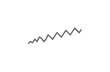
\begin{tikzpicture}[x=0.08em, y=0.08em, line width=0.4pt]
                \draw[FooterGray] (0,3) -- (1,4) -- (2,3.5) -- (3,5) -- (4,4) -- (5,6) -- (6,5.5) -- (7,4) -- (8,5) -- (9,7) -- (10,6) -- (11,5) -- (12,6.5) -- (13,8) -- (14,7) -- (15,6) -- (16,7.5) -- (17,9) -- (18,8) -- (19,7) -- (20,8.5) -- (21,10) -- (22,9) -- (23,8) -- (24,9.5);
            \end{tikzpicture}%
        }%
        \hskip0.5cm%
    }%
    \vskip6pt%
}

%=============================================================================
% PACKAGES
%=============================================================================
\usepackage[utf8]{inputenc}
\usepackage[T1]{fontenc}
\usepackage{amsmath, amssymb, amsthm}
\usepackage{mathtools}
\usepackage{bm}
\usepackage{tikz}
\usetikzlibrary{arrows.meta, positioning, shapes, calc, decorations.pathreplacing, shadings}
\usepackage{booktabs}
\usepackage{multirow}
\usepackage{array}
\usepackage{graphicx}
\usepackage{hyperref}
\usepackage{colortbl}
\hypersetup{colorlinks=true, linkcolor=MainBlue, urlcolor=MainBlue}
\graphicspath{{../../logos/}{../../charts/}{../../photos/}}
\hfuzz=2pt  % Suppress tiny overfull warnings (<2pt)
\vfuzz=2pt  % Suppress tiny vertical overfull warnings (<2pt)

%=============================================================================
% QUANTLET COMMAND
%=============================================================================
\newcommand{\quantlet}[2]{%
    \hfill\href{#2}{%
        \raisebox{-0.15em}{\includegraphics[height=0.7em]{ql_logo.png}}%
        \textcolor{MainBlue}{\tiny\ #1}%
    }%
}

%=============================================================================
% CUSTOM TITLE PAGE
%=============================================================================
\defbeamertemplate*{title page}{hybrid}[1][]
{
    \vspace{0.2cm}
    % Logos row - top header (with clickable links)
    \begin{center}
        \href{https://www.ase.ro}{\includegraphics[height=1.0cm]{ase_logo.png}}\hspace{0.3cm}%
        \href{https://theida.net}{\includegraphics[height=1.0cm]{ida_logo.png}}\hspace{0.3cm}%
        \href{https://blockchain-research-center.com}{\includegraphics[height=1.0cm]{brc_logo.png}}\hspace{0.3cm}%
        \href{https://www.ai4efin.ase.ro}{\includegraphics[height=1.0cm]{ai4efin_logo.png}}\hspace{0.3cm}%
        \href{https://ipe.ro/new}{\includegraphics[height=1.0cm]{acad_logo.png}}\hspace{0.3cm}%
        \href{https://www.digital-finance-msca.com}{\includegraphics[height=1.0cm]{msca_logo.png}}%
    \end{center}

    \vspace{0.6cm}

    % Main title with Q logos on sides (with clickable links)
    \begin{center}
        \begin{minipage}{0.1\textwidth}
            \centering
            \href{https://quantlet.com}{\includegraphics[height=1.1cm]{ql_logo.png}}
        \end{minipage}%
        \begin{minipage}{0.78\textwidth}
            \centering
            {\LARGE\bfseries\usebeamercolor[fg]{title}\inserttitle}

            \vspace{0.3cm}

            {\usebeamerfont{subtitle}\usebeamercolor[fg]{title}\insertsubtitle}
        \end{minipage}%
        \begin{minipage}{0.1\textwidth}
            \centering
            \href{https://quantinar.com}{\includegraphics[height=1.1cm]{qr_logo.png}}
        \end{minipage}
    \end{center}

    \vspace{0.6cm}

    % Authors (left aligned)
    \hspace{0.5cm}{\usebeamerfont{author}\insertauthor}

    \vspace{0.3cm}

    % Institute/Affiliations (left aligned)
    \hspace{0.5cm}\begin{minipage}[t]{0.9\textwidth}
        \raggedright\small\insertinstitute
    \end{minipage}
}

%=============================================================================
% THEOREM ENVIRONMENTS
%=============================================================================
\theoremstyle{definition}
\setbeamertemplate{theorems}[numbered]
\newtheorem{defn}{Definition}
\newtheorem{thm}{Theorem}
\newtheorem{prop}{Proposition}
\newtheorem{rmk}{Remark}

%=============================================================================
% CENTRED MINIPAGE (no extra vertical space)
%=============================================================================
\newenvironment{cminipage}[1]{%
    \par\noindent\hfill\begin{minipage}{#1}\ignorespaces
}{%
    \end{minipage}\hfill\null\par
}

%=============================================================================
% CUSTOM COMMANDS
%=============================================================================
\newcommand{\E}{\mathbb{E}}
\newcommand{\Var}{\text{Var}}
\newcommand{\Cov}{\text{Cov}}
\newcommand{\Corr}{\text{Corr}}
\newcommand{\R}{\mathbb{R}}
\newcommand{\N}{\mathbb{N}}
\newcommand{\Z}{\mathbb{Z}}
\newcommand{\B}{\mathbf{B}}
\newcommand{\imark}{\textcolor{MainBlue}{\textbullet}}
\newcommand{\RMSE}{\text{RMSE}}
\newcommand{\MAE}{\text{MAE}}
\newcommand{\MAPE}{\text{MAPE}}

%=============================================================================
% TITLE INFORMATION
%=============================================================================
\title[Time Series Analysis]{Time Series Analysis and Forecasting}
\subtitle{Chapter 5: GARCH and Volatility}
\author[D.T. Pele]{Daniel Traian PELE}
\institute{Bucharest University of Economic Studies\\
IDA Institute Digital Assets\\
Blockchain Research Center\\
AI4EFin Artificial Intelligence for Energy Finance\\
Romanian Academy, Institute for Economic Forecasting\\
MSCA Digital Finance}
\date{}

\begin{document}

% Title page (no header/footer)
{
\setbeamertemplate{headline}{}
\setbeamertemplate{footline}{}
\begin{frame}
    \titlepage
\end{frame}
}

%=============================================================================
% TABLE OF CONTENTS
%=============================================================================
\begin{frame}{Outline}
    \vspace{-0.3cm}
    {\small
    \begin{columns}[T]
        \begin{column}{0.48\textwidth}
            \begin{block}{Foundations}
                \begin{itemize}\setlength{\itemsep}{3pt}
                    \item Motivation
                    \item Introduction to Volatility Modeling
                    \item The ARCH Model
                    \item The GARCH Model
                    \item Asymmetric GARCH Models
                    \item Model Selection and Diagnostics
                \end{itemize}
            \end{block}
        \end{column}
        \begin{column}{0.48\textwidth}
            \begin{exampleblock}{Applications}
                \begin{itemize}\setlength{\itemsep}{3pt}
                    \item Volatility Forecasting
                    \item Python Implementation
                    \item Case Study: S\&P 500
                    \item Case Study: Bitcoin
                    \item Summary and Quiz
                \end{itemize}
            \end{exampleblock}
        \end{column}
    \end{columns}
    }
\end{frame}

%=============================================================================
% LEARNING OBJECTIVES
%=============================================================================
\section{Motivation}

\begin{frame}{Learning Objectives}
    \begin{cminipage}{0.95\textwidth}
\begin{block}{By the end of this chapter, you will be able to:}
\begin{enumerate}\setlength{\itemsep}{0pt}
    \item Understand \textbf{volatility clustering} and stylized facts of financial returns
    \item Estimate and interpret \textbf{ARCH} and \textbf{GARCH} models
    \item Apply asymmetric models (\textbf{EGARCH}, \textbf{GJR-GARCH}) for the leverage effect
    \item Perform model validation and selection
    \item Forecast volatility and calculate \textbf{Value at Risk (VaR)}
\end{enumerate}
\end{block}
\vspace{-0.1cm}
\begin{alertblock}{Practical Skills}
    \begin{itemize}\setlength{\itemsep}{0pt}
        \item Python implementation with the \texttt{arch} package
            \begin{itemize}\setlength{\itemsep}{0pt}
                \item Estimation, forecasting, and automatic diagnostics
            \end{itemize}
        \item Interpreting parameters and volatility persistence
        \item VaR calculation for risk management
            \begin{itemize}\setlength{\itemsep}{0pt}
                \item Backtesting and forecast validation
            \end{itemize}
    \end{itemize}
\end{alertblock}
    \end{cminipage}
\end{frame}

%=============================================================================
% SECTION 1: INTRODUCTION TO VOLATILITY
%=============================================================================
\section{Introduction to Volatility Modeling}

\begin{frame}{Volatility Clustering}
    \vspace{-0.2cm}
    {\scriptsize
    \begin{itemize}\setlength{\itemsep}{0pt}
        \item High volatility periods are followed by high volatility; calm by calm
        \item This suggests that \textbf{conditional variance} is predictable
    \end{itemize}
    }
    \begin{center}
        \includegraphics[width=0.95\textwidth, height=0.50\textheight, keepaspectratio]{garch_volatility_clustering.pdf}
    \end{center}
    \quantlet{TSA\_ch5\_clustering}{https://github.com/QuantLet/TSA/tree/main/TSA_ch5/TSA_ch5_clustering}
\end{frame}

\begin{frame}{Why Model Volatility?}
    \begin{cminipage}{0.95\textwidth}
    \small
    \begin{block}{Empirical Observations in Financial Series}
        \begin{itemize}\setlength{\itemsep}{0pt}
            \item Financial returns exhibit \textbf{volatility clustering} --- periods of high volatility tend to be followed by periods of high volatility
            \item The distribution of returns has \textbf{fat tails} (leptokurtosis)
            \item Return correlation is nearly zero, but correlation of squares is significant
            \item Volatility responds \textbf{asymmetrically} to shocks (leverage effect)
        \end{itemize}
    \end{block}

    \vspace{0.3cm}

    \begin{alertblock}{Limitation of ARIMA Models}
        ARIMA models assume \textbf{constant variance} (homoskedasticity), which is not realistic for financial series!
    \end{alertblock}
    \end{cminipage}
\end{frame}

\begin{frame}{Example: Bitcoin $\succ$ Volatility Clustering}
    \vspace{-0.2cm}
    \begin{center}
        \includegraphics[width=0.95\textwidth, height=0.47\textheight, keepaspectratio]{btc_returns.pdf}
    \end{center}
    \vspace{-0.2cm}
    {\footnotesize
    \begin{block}{Observations}
        \begin{itemize}\setlength{\itemsep}{0pt}
            \item Bitcoin daily returns (2019--2025): extremely pronounced volatility clustering
                \begin{itemize}\setlength{\itemsep}{0pt}
                    \item Returns of $\pm 20\%$ during crisis periods (COVID, Terra/Luna)
                \end{itemize}
            \item Bitcoin volatility is significantly higher than traditional assets
                \begin{itemize}\setlength{\itemsep}{0pt}
                    \item Typical $\alpha \approx 0.10$--$0.20$ (fast reaction to news)
                \end{itemize}
        \end{itemize}
    \end{block}
    }
    \quantlet{TSA\_ch5\_btc\_returns}{https://github.com/QuantLet/TSA/tree/main/TSA_ch5/TSA_ch5_btc_returns}
\end{frame}

\begin{frame}{Stylized Facts of Financial Returns}
    \vspace{-0.2cm}
    \begin{columns}[T]
        \column{0.55\textwidth}
        {\scriptsize
        \begin{block}{Observed Properties}
            \begin{enumerate}\setlength{\itemsep}{0pt}
                \item \textbf{No autocorrelation} in returns
                \item \textbf{Autocorrelation} in $r_t^2$, $|r_t|$
                \item \textbf{Fat tails} (kurtosis $> 3$)
                \item \textbf{Leverage effect}
                \item \textbf{Volatility clustering}
            \end{enumerate}
        \end{block}
        }
        \column{0.43\textwidth}
        \vspace{-0.3cm}
        \begin{center}
            \includegraphics[width=\textwidth, keepaspectratio]{garch_stylized_facts.pdf}
        \end{center}
        \quantlet{TSA\_ch5\_stylized}{https://github.com/QuantLet/TSA/tree/main/TSA_ch5/TSA_ch5_stylized}
    \end{columns}
\end{frame}

\begin{frame}{Example: Bitcoin $\succ$ Evidence for ARCH Effects}
    \vspace{-0.2cm}
    \begin{center}
        \includegraphics[width=0.95\textwidth, height=0.31\textheight, keepaspectratio]{btc_acf_squared.pdf}
    \end{center}
    \vspace{-0.2cm}
    {\scriptsize
    \small
    \begin{defn}[Conditional Variance]
        For return series $\{r_t\}$, the \textbf{conditional variance} at time $t$ is:
        $\sigma_t^2 = \Var(r_t | \mathcal{F}_{t-1}) = \E[(r_t - \mu_t)^2 | \mathcal{F}_{t-1}]$
        where $\mathcal{F}_{t-1}$ is the information available up to time $t-1$.
    \end{defn}

    \vspace{0.05cm}

    \begin{block}{General Model}
        $r_t = \mu_t + \varepsilon_t$, \quad $\varepsilon_t = \sigma_t z_t$, \quad $z_t \sim \text{i.i.d.}(0, 1)$
        \begin{itemize}\setlength{\itemsep}{0pt}
            \item $\mu_t$ = conditional mean (ARMA); \quad $\sigma_t^2$ = conditional variance (GARCH)
            \item $z_t$ = standardized innovations (Normal, Student-t, GED)
        \end{itemize}
    \end{block}
    }
    \quantlet{TSA\_ch5\_btc\_arch}{https://github.com/QuantLet/TSA/tree/main/TSA_ch5/TSA_ch5_btc_arch}
\end{frame}

%=============================================================================
% SECTION 2: ARCH MODEL
%=============================================================================
\section{The ARCH Model}

\begin{frame}{Researcher Spotlight: Engle \& Bollerslev}
    \vspace{-0.2cm}
    \begin{columns}[T]
        \begin{column}{0.22\textwidth}
            \centering
            \includegraphics[width=0.95\textwidth, height=0.22\textheight, keepaspectratio]{photo_robert_engle.jpg}
            \\[0.05cm]
            {\tiny\textcolor{MediumGray}{Robert Engle (*1942)}}\\[-0.05cm]
            {\tiny\textcolor{MediumGray}{Nobel Prize 2003}}\\[0.02cm]
            \href{https://en.wikipedia.org/wiki/Robert_F._Engle}{\faWikipediaW\ \textcolor{MainBlue}{\tiny Wikipedia}}
        \end{column}
        \begin{column}{0.76\textwidth}
            \begin{block}{Biography}
                {\footnotesize \begin{itemize}\setlength{\itemsep}{0pt}
                    \item \textbf{Robert Engle}: American economist at NYU Stern. Nobel Prize (2003) ``for methods of analyzing economic time series with time-varying volatility (ARCH)''
                    \item \textbf{Tim Bollerslev}: Danish-American economist at Duke University, PhD student of Engle
                \end{itemize}}
            \end{block}
        \end{column}
    \end{columns}
    \vspace{0.1cm}
    \begin{columns}[T]
        \begin{column}{0.22\textwidth}
            \centering
            \includegraphics[width=0.95\textwidth, height=0.22\textheight, keepaspectratio]{photo_tim_bollerslev.jpg}
            \\[0.05cm]
            {\tiny\textcolor{MediumGray}{Tim Bollerslev (*1958)}}\\[0.02cm]
            \href{https://en.wikipedia.org/wiki/Tim_Bollerslev}{\faWikipediaW\ \textcolor{MainBlue}{\tiny Wikipedia}}
        \end{column}
        \begin{column}{0.76\textwidth}
            \begin{exampleblock}{Key Contributions}
                {\footnotesize
                \begin{itemize}\setlength{\itemsep}{0pt}
                    \item \textbf{ARCH model} (Engle, 1982) --- autoregressive conditional heteroskedasticity
                    \item \textbf{GARCH model} (Bollerslev, 1986) --- generalized ARCH with persistent volatility
                    \item \textbf{Realized volatility} measures and high-frequency econometrics
                    \item Foundation for modern financial risk management (VaR, ES)
                \end{itemize}}
            \end{exampleblock}
        \end{column}
    \end{columns}
\end{frame}

\begin{frame}{ARCH(1) Simulation: Effect of $\alpha$ Parameter}
    \vspace{-0.2cm}
    {\scriptsize
    \begin{block}{Interpretation}
        \begin{itemize}\setlength{\itemsep}{0pt}
            \item Higher $\alpha$ means volatility reacts more strongly to recent shocks
        \end{itemize}
    \end{block}
    }
    \begin{center}
        \includegraphics[width=0.95\textwidth, height=0.50\textheight, keepaspectratio]{garch_arch1_simulation.pdf}
    \end{center}
    \quantlet{TSA\_ch5\_arch\_sim}{https://github.com/QuantLet/TSA/tree/main/TSA_ch5/TSA_ch5_arch_sim}
\end{frame}

\begin{frame}{The ARCH(q) Model --- Engle (1982)}
    \begin{cminipage}{0.95\textwidth}
    \small
    \begin{defn}[ARCH(q)]
        The \textbf{Autoregressive Conditional Heteroskedasticity} model of order $q$:
        \[
            \varepsilon_t = \sigma_t z_t, \quad z_t \sim \text{i.i.d.}(0, 1), \quad
            \sigma_t^2 = \omega + \sum_{i=1}^{q} \alpha_i \varepsilon_{t-i}^2
        \]
    \end{defn}

    \vspace{0.2cm}

    \begin{block}{Stationarity Restrictions}
        \begin{itemize}\setlength{\itemsep}{0pt}
            \item $\omega > 0$ (positive base variance), \quad $\alpha_i \geq 0$ (non-negativity)
            \item $\sum_{i=1}^{q} \alpha_i < 1$ (stationarity)
        \end{itemize}
    \end{block}

    \begin{rmk}
        Robert Engle received the \textbf{Nobel Prize in Economics} in 2003 for developing the ARCH model!
    \end{rmk}
    \end{cminipage}
\end{frame}

\begin{frame}{Properties of the ARCH(1) Model}
    \begin{cminipage}{0.95\textwidth}
    \begin{block}{ARCH(1): $\sigma_t^2 = \omega + \alpha_1 \varepsilon_{t-1}^2$}
        \begin{itemize}\setlength{\itemsep}{0pt}
            \item \textbf{Unconditional variance}: $\E[\varepsilon_t^2] = \dfrac{\omega}{1 - \alpha_1}$ (if $\alpha_1 < 1$)
            \item \textbf{Kurtosis}: $\kappa = 3 \cdot \dfrac{1 - \alpha_1^2}{1 - 3\alpha_1^2}$ (if $\alpha_1^2 < 1/3$)
            \item Kurtosis $> 3$ for $\alpha_1 > 0$ $\Rightarrow$ \textbf{fat tails}!
        \end{itemize}
    \end{block}

    \vspace{0.3cm}

    \begin{exampleblock}{Numerical Example}
        If $\omega = 0.0001$ and $\alpha_1 = 0.3$:
        \begin{itemize}\setlength{\itemsep}{0pt}
            \item Unconditional variance: $\sigma^2 = \frac{0.0001}{1 - 0.3} = 0.000143$
            \item Kurtosis: $\kappa = 3 \cdot \frac{1 - 0.09}{1 - 0.27} = 3.74 > 3$
        \end{itemize}
    \end{exampleblock}
    \end{cminipage}
\end{frame}

\begin{frame}{Derivation: Unconditional Variance of ARCH(1)}
    \begin{cminipage}{0.95\textwidth}
    \begin{proof}[Derivation]
        Let $\varepsilon_t = \sigma_t z_t$ with $z_t \sim N(0,1)$ and $\sigma_t^2 = \omega + \alpha_1 \varepsilon_{t-1}^2$.

        \vspace{0.2cm}
        \textbf{Step 1}: Take unconditional expectation:
        \[
            \E[\varepsilon_t^2] = \E[\sigma_t^2 z_t^2] = \E[\sigma_t^2] \cdot \E[z_t^2] = \E[\sigma_t^2]
        \]

        \textbf{Step 2}: Apply expectation to variance equation:
        \[
            \E[\sigma_t^2] = \E[\omega + \alpha_1 \varepsilon_{t-1}^2] = \omega + \alpha_1 \E[\varepsilon_{t-1}^2]
        \]

        \textbf{Step 3}: By stationarity, $\E[\varepsilon_t^2] = \E[\varepsilon_{t-1}^2] = \sigma^2$:
        \[
            \sigma^2 = \omega + \alpha_1 \sigma^2 \quad \Rightarrow \quad \sigma^2 (1 - \alpha_1) = \omega
        \]

        \textbf{Result}: $\boxed{\sigma^2 = \dfrac{\omega}{1 - \alpha_1}}$ \quad (requires $\alpha_1 < 1$ for stationarity)
    \end{proof}
    \end{cminipage}
\end{frame}

\begin{frame}{Derivation: Kurtosis of ARCH(1)}
    \begin{cminipage}{0.95\textwidth}
    {\small
    For $\varepsilon_t = \sigma_t z_t$ with $z_t \sim N(0,1)$:

    \textbf{Step 1}: $\E[\varepsilon_t^4] = \E[\sigma_t^4] \cdot \E[z_t^4] = 3 \E[\sigma_t^4]$ \quad (since $\E[z^4] = 3$)

    \textbf{Step 2}: Using $\sigma_t^2 = \omega + \alpha_1 \varepsilon_{t-1}^2$:
    \[
        \E[\sigma_t^4] = \E[(\omega + \alpha_1 \varepsilon_{t-1}^2)^2] = \omega^2 + 2\omega\alpha_1 \sigma^2 + \alpha_1^2 \E[\varepsilon_{t-1}^4]
    \]

    \textbf{Step 3}: Solving the recursion yields:
    \[
        \boxed{\kappa = \frac{\E[\varepsilon_t^4]}{(\E[\varepsilon_t^2])^2} = 3 \cdot \frac{1 - \alpha_1^2}{1 - 3\alpha_1^2}}
    \]
    }

    \begin{block}{Interpretation}
        \begin{itemize}\setlength{\itemsep}{0pt}
            \item $\kappa > 3$ for any $\alpha_1 > 0$ $\Rightarrow$ \textbf{fat tails} (leptokurtosis)
            \item Requires $\alpha_1 < 0.577$ for finite fourth moment
            \item ARCH naturally generates heavy-tailed distributions!
        \end{itemize}
    \end{block}
    \end{cminipage}
\end{frame}

\begin{frame}{Testing for ARCH Effects}
    \begin{cminipage}{0.95\textwidth}
    \begin{block}{Engle's Test for ARCH Effects}
        \textbf{Procedure}:
        \begin{enumerate}\setlength{\itemsep}{0pt}
            \item Estimate the mean model and obtain residuals $\hat{\varepsilon}_t$
            \item Calculate $\hat{\varepsilon}_t^2$
            \item Regress $\hat{\varepsilon}_t^2$ on its lags:
            \[
                \hat{\varepsilon}_t^2 = \beta_0 + \beta_1 \hat{\varepsilon}_{t-1}^2 + \cdots + \beta_q \hat{\varepsilon}_{t-q}^2 + u_t
            \]
            \item Calculate the statistic $LM = T \cdot R^2 \sim \chi^2(q)$
        \end{enumerate}
    \end{block}

    \vspace{0.3cm}

    \begin{alertblock}{Hypotheses}
        \begin{itemize}\setlength{\itemsep}{0pt}
            \item $H_0$: No ARCH effects ($\alpha_1 = \cdots = \alpha_q = 0$)
            \item $H_1$: ARCH effects present (at least one $\alpha_i \neq 0$)
        \end{itemize}
    \end{alertblock}
    \end{cminipage}
\end{frame}

\begin{frame}{Limitations of the ARCH Model}
    \begin{cminipage}{0.95\textwidth}
    \begin{alertblock}{Practical Problems}
        \begin{enumerate}\setlength{\itemsep}{0pt}
            \item \textbf{High order} --- many lags are usually needed (large $q$)
            \item \textbf{Many parameters} --- estimation difficulties
            \item \textbf{Non-negativity constraints} --- difficult to impose for large $q$
            \item \textbf{Does not capture persistence} --- observed volatility is very persistent
        \end{enumerate}
    \end{alertblock}

    \vspace{0.5cm}

    \begin{block}{The Solution}
        \textbf{The GARCH Model} --- introduces lags of conditional variance to capture persistence with fewer parameters!
    \end{block}
    \end{cminipage}
\end{frame}

%=============================================================================
% SECTION 3: GARCH MODEL
%=============================================================================
\section{The GARCH Model}

\begin{frame}{The GARCH(1,1) Model}
    \vspace{-0.2cm}
    \begin{columns}[T]
        \column{0.55\textwidth}
        {\scriptsize
        \begin{cminipage}{0.95\textwidth}
        \small
        \begin{block}{The Most Popular Volatility Model}
            $\sigma_t^2 = \omega + \alpha \varepsilon_{t-1}^2 + \beta \sigma_{t-1}^2$
        \end{block}

        \vspace{0.3cm}
        \vspace{-0.1cm}
        \begin{block}{Restrictions \& Properties}
            \begin{itemize}\setlength{\itemsep}{0pt}
                \item $\omega > 0$, $\alpha \geq 0$, $\beta \geq 0$; \quad $\alpha + \beta < 1$ (stationarity)
                \item $\bar{\sigma}^2 = \frac{\omega}{1 - \alpha - \beta}$; \quad Half-life: $HL = \frac{\ln(0.5)}{\ln(\alpha + \beta)}$
            \end{itemize}
        \end{block}
        \end{cminipage}
        }
        \column{0.43\textwidth}
        \vspace{-0.3cm}
        \begin{center}
            \includegraphics[width=\textwidth, keepaspectratio]{garch_conditional_variance.pdf}
        \end{center}
    \end{columns}
\end{frame}

\begin{frame}{The GARCH(p,q) Model --- Bollerslev (1986)}
    \begin{cminipage}{0.95\textwidth}
    \small
    \begin{defn}[GARCH(p,q)]
        The \textbf{Generalized ARCH} model:
        \[
            \varepsilon_t = \sigma_t z_t, \quad z_t \sim \text{i.i.d.}(0, 1)
        \]
        \[
            \sigma_t^2 = \omega + \sum_{i=1}^{q} \alpha_i \varepsilon_{t-i}^2 + \sum_{j=1}^{p} \beta_j \sigma_{t-j}^2
        \]
    \end{defn}

    \vspace{0.3cm}

    \begin{block}{Interpretation}
        \begin{itemize}\setlength{\itemsep}{0pt}
            \item $\omega$ = base level of volatility
            \item $\alpha_i$ = reaction to recent shocks (news coefficients)
            \item $\beta_j$ = volatility persistence (memory)
            \item $\alpha + \beta$ = total persistence
        \end{itemize}
    \end{block}
    \end{cminipage}
\end{frame}

\begin{frame}{GARCH(1,1) Simulation: Persistence Effect}
    \vspace{-0.2cm}
    \begin{columns}[T]
        \column{0.55\textwidth}
        {\scriptsize
        \begin{cminipage}{0.95\textwidth}
        \vspace{-0.2cm}
        {\footnotesize
        \begin{block}{Interpretation}
            \begin{itemize}\setlength{\itemsep}{0pt}
                \item $\alpha$ controls reaction to shocks
                \item $\beta$ controls persistence
                \item The sum $\alpha + \beta$ determines mean-reversion speed
            \end{itemize}
        \end{block}
        }
        \end{cminipage}
        }
        \column{0.43\textwidth}
        \vspace{-0.3cm}
        \begin{center}
            \includegraphics[width=\textwidth, keepaspectratio]{garch_garch11_simulation.pdf}
        \end{center}
        \quantlet{TSA\_ch5\_garch\_sim}{https://github.com/QuantLet/TSA/tree/main/TSA_ch5/TSA_ch5_garch_sim}
    \end{columns}
\end{frame}

\begin{frame}{Derivation: Unconditional Variance of GARCH(1,1)}
\small
    \begin{proof}[Derivation]
        For $\sigma_t^2 = \omega + \alpha \varepsilon_{t-1}^2 + \beta \sigma_{t-1}^2$:

        \textbf{Step 1}: Take unconditional expectation:
        $\E[\sigma_t^2] = \omega + \alpha \E[\varepsilon_{t-1}^2] + \beta \E[\sigma_{t-1}^2]$

        \textbf{Step 2}: By stationarity, $\E[\sigma_t^2] = \E[\sigma_{t-1}^2] = \bar{\sigma}^2$ and $\E[\varepsilon_t^2] = \bar{\sigma}^2$:
        $\bar{\sigma}^2 = \omega + (\alpha + \beta) \bar{\sigma}^2$

        \textbf{Step 3}: Solve: $\bar{\sigma}^2 (1 - \alpha - \beta) = \omega \Rightarrow \boxed{\bar{\sigma}^2 = \frac{\omega}{1 - \alpha - \beta}}$
    \end{proof}
    \vspace{-0.1cm}
    \begin{alertblock}{Stationarity Condition}
        Requires $\alpha + \beta < 1$ for finite unconditional variance.
    \end{alertblock}
\end{frame}

\begin{frame}{GARCH(1,1) as ARMA for $\varepsilon_t^2$}
    \vspace{-0.2cm}
    {\footnotesize
    \begin{block}{ARMA(1,1) Representation}
        Define $\nu_t = \varepsilon_t^2 - \sigma_t^2$ (variance shock). Then:
        \[
            \varepsilon_t^2 = \omega + (\alpha + \beta) \varepsilon_{t-1}^2 + \nu_t - \beta \nu_{t-1}
        \]

        This is an \textbf{ARMA(1,1)} for $\varepsilon_t^2$!
    \end{block}

    \vspace{0.3cm}

    \begin{exampleblock}{Implications}
        \begin{itemize}\setlength{\itemsep}{0pt}
            \item ACF of $\varepsilon_t^2$ decays exponentially (like ARMA)
            \item Persistence is given by $\alpha + \beta$
            \item PACF can help identify the order
        \end{itemize}
    \end{exampleblock}
    }
\end{frame}

\begin{frame}{Derivation: ARMA Representation of GARCH(1,1)}
    \begin{proof}[Derivation]
        \textbf{Step 1}: Define variance shock: $\nu_t = \varepsilon_t^2 - \sigma_t^2$
        \begin{itemize}
            \item $\E[\nu_t | \mathcal{F}_{t-1}] = \E[\varepsilon_t^2 | \mathcal{F}_{t-1}] - \sigma_t^2 = \sigma_t^2 - \sigma_t^2 = 0$
            \item $\nu_t$ is a martingale difference sequence
        \end{itemize}

        \vspace{0.2cm}
        \textbf{Step 2}: Substitute $\sigma_t^2 = \varepsilon_t^2 - \nu_t$ into GARCH equation:
        \[
            \varepsilon_t^2 - \nu_t = \omega + \alpha \varepsilon_{t-1}^2 + \beta (\varepsilon_{t-1}^2 - \nu_{t-1})
        \]

        \textbf{Step 3}: Rearrange:
        \[
            \varepsilon_t^2 = \omega + (\alpha + \beta) \varepsilon_{t-1}^2 + \nu_t - \beta \nu_{t-1}
        \]

        \textbf{Result}: ARMA(1,1) with AR coefficient $\phi = \alpha + \beta$ and MA coefficient $\theta = -\beta$.
    \end{proof}
\end{frame}

\begin{frame}{Derivation: Volatility Persistence and Half-Life}
    \begin{cminipage}{0.95\textwidth}
\small
    \begin{block}{Multi-Step Forecast GARCH(1,1)}
        \begin{itemize}\setlength{\itemsep}{0pt}
            \item $\E_t[\sigma_{t+h}^2] = \bar{\sigma}^2 + (\alpha+\beta)^{h-1}(\sigma_{t+1}^2 - \bar{\sigma}^2)$
        \end{itemize}
    \end{block}
    \vspace{-0.1cm}
    \begin{block}{Derivation}
        \begin{itemize}\setlength{\itemsep}{0pt}
            \item \textbf{Step 1}: Let $\phi = \alpha + \beta$ and $q_t = \sigma_t^2 - \bar{\sigma}^2$ (deviation from mean)
            \item \textbf{Step 2}: From the GARCH equation: $\E_t[q_{t+1}] = \phi \cdot q_t$, so $\E_t[q_{t+h}] = \phi^h \cdot q_t$
            \item \textbf{Step 3}: Half-life = time until deviation halves:
            $\phi^{HL} = 0.5 \;\Rightarrow\; HL = \frac{\ln(0.5)}{\ln(\phi)} = \frac{-0.693}{\ln(\alpha+\beta)}$
        \end{itemize}
    \end{block}
    \vspace{-0.1cm}
    \begin{exampleblock}{Example: S\&P 500}
        \begin{itemize}\setlength{\itemsep}{0pt}
            \item With $\alpha + \beta = 0.988$: $HL = \frac{-0.693}{-0.012} \approx \textbf{58 days}$ (shocks persist $\sim$3 months!)
        \end{itemize}
    \end{exampleblock}
    \end{cminipage}
\end{frame}

\begin{frame}{Estimation of GARCH Models}
    \begin{cminipage}{0.95\textwidth}
    \small
    \begin{block}{Maximum Likelihood Estimation (MLE)}
        Log-likelihood (normal): $\ell(\theta) = -\frac{T}{2} \ln(2\pi) - \frac{1}{2} \sum_{t=1}^{T} \left[ \ln(\sigma_t^2) + \frac{\varepsilon_t^2}{\sigma_t^2} \right]$
    \end{block}

    \vspace{0.2cm}

    \begin{block}{Alternative Distributions for $z_t$}
        \begin{itemize}\setlength{\itemsep}{0pt}
            \item \textbf{Student-t}: captures fat tails --- most common choice
            \item \textbf{GED}: flexibility for kurtosis
            \item \textbf{Skewed Student-t}: asymmetry and fat tails
        \end{itemize}
    \end{block}

    \vspace{0.2cm}

    \begin{alertblock}{Practical Note}
        Student-t distribution typically provides better fit for financial returns due to fat tails (kurtosis $> 3$).
    \end{alertblock}
    \end{cminipage}
\end{frame}

\begin{frame}{Typical Values for GARCH(1,1)}
    \begin{cminipage}{0.95\textwidth}
    \begin{center}
        \begin{tabular}{lccc}
            \toprule
            \textbf{Series} & $\bm{\alpha}$ & $\bm{\beta}$ & $\bm{\alpha + \beta}$ \\
            \midrule
            S\&P 500 daily & 0.05--0.10 & 0.85--0.95 & 0.95--0.99 \\
            EUR/USD daily & 0.03--0.08 & 0.90--0.95 & 0.95--0.99 \\
            Bitcoin daily & 0.10--0.20 & 0.75--0.85 & 0.90--0.98 \\
            Bonds & 0.02--0.05 & 0.90--0.97 & 0.95--0.99 \\
            \bottomrule
        \end{tabular}
    \end{center}

    \vspace{0.5cm}

    \begin{alertblock}{Observations}
        \begin{itemize}\setlength{\itemsep}{0pt}
            \item $\alpha + \beta$ close to 1 $\Rightarrow$ \textbf{very persistent volatility}
            \item Small $\alpha$, large $\beta$ $\Rightarrow$ slow reaction to shocks, long memory
            \item Bitcoin: larger $\alpha$ $\Rightarrow$ faster reaction to news
        \end{itemize}
    \end{alertblock}
    \end{cminipage}
\end{frame}

\begin{frame}{GARCH vs IGARCH: Persistence Comparison}
    \vspace{-0.2cm}
    {\scriptsize
    \begin{block}{Interpretation}
        \begin{itemize}\setlength{\itemsep}{0pt}
            \item Standard GARCH reverts to unconditional mean
            \item IGARCH has no finite mean $\Rightarrow$ shocks persist indefinitely
        \end{itemize}
    \end{block}
    }
    \begin{center}
        \includegraphics[width=0.95\textwidth, height=0.50\textheight, keepaspectratio]{garch_igarch_comparison.pdf}
    \end{center}
    \quantlet{TSA\_ch5\_igarch}{https://github.com/QuantLet/TSA/tree/main/TSA_ch5/TSA_ch5_igarch}
\end{frame}

\begin{frame}{IGARCH --- Integrated GARCH}
    \begin{cminipage}{0.95\textwidth}
    \small
    \begin{defn}[IGARCH(1,1)]
        When $\alpha + \beta = 1$:
        \[
            \sigma_t^2 = \omega + \alpha \varepsilon_{t-1}^2 + (1 - \alpha) \sigma_{t-1}^2
        \]
    \end{defn}

    \vspace{0.3cm}

    \begin{block}{Properties}
        \begin{itemize}\setlength{\itemsep}{0pt}
            \item Unconditional variance does not exist (infinite)
            \item Shocks have \textbf{permanent} effect on volatility
            \item Used for series with extreme persistence
            \item Useful for \textbf{RiskMetrics} (J.P. Morgan): $\alpha = 0.06$, $\beta = 0.94$
        \end{itemize}
    \end{block}

    \begin{rmk}
        IGARCH is analogous to a unit root in variance!
    \end{rmk}
    \end{cminipage}
\end{frame}

%=============================================================================
% SECTION 4: ASYMMETRIC GARCH MODELS
%=============================================================================
\section{Asymmetric GARCH Models}

\begin{frame}{Leverage Effect}
    \vspace{-0.2cm}
    \begin{columns}[T]
        \column{0.55\textwidth}
        {\scriptsize
        \begin{cminipage}{0.95\textwidth}
        \vspace{0.3cm}
        \vspace{-0.1cm}
        \small
        \begin{block}{Definition}
            \textbf{Leverage effect}: Negative shocks increase volatility \textbf{more} than positive shocks of the same magnitude.
        \end{block}
        \begin{alertblock}{Problem with GARCH}
            Standard GARCH: $\sigma_t^2 = \omega + \alpha \varepsilon_{t-1}^2 + \beta \sigma_{t-1}^2$ --- only $\varepsilon_{t-1}^2$ matters, sign is lost! Economic intuition: Bad news $\Rightarrow$ stock price falls $\Rightarrow$ debt/equity ratio rises $\Rightarrow$ volatility increases.
        \end{alertblock}
        \end{cminipage}
        }
        \column{0.43\textwidth}
        \vspace{-0.3cm}
        \begin{center}
            \includegraphics[width=\textwidth, keepaspectratio]{garch_leverage_effect.pdf}
        \end{center}
    \end{columns}
\end{frame}

\begin{frame}{EGARCH Simulation: Symmetric vs Asymmetric}
    \vspace{-0.2cm}
    {\scriptsize
    \begin{block}{Interpretation}
        \begin{itemize}\setlength{\itemsep}{0pt}
            \item When $\gamma < 0$, negative shocks increase volatility more than positive shocks
        \end{itemize}
    \end{block}
    }
    \begin{center}
        \includegraphics[width=0.95\textwidth, height=0.50\textheight, keepaspectratio]{garch_egarch_simulation.pdf}
    \end{center}
    \quantlet{TSA\_ch5\_egarch\_sim}{https://github.com/QuantLet/TSA/tree/main/TSA_ch5/TSA_ch5_egarch_sim}
\end{frame}

\begin{frame}{The EGARCH Model --- Nelson (1991)}
    \begin{cminipage}{0.95\textwidth}
    \vspace{-0.3cm}
    {\footnotesize
    \begin{defn}[EGARCH(1,1)]
        \textbf{Exponential GARCH}:
        \[
            \ln(\sigma_t^2) = \omega + \alpha \left( |z_{t-1}| - \E[|z_{t-1}|] \right) + \gamma z_{t-1} + \beta \ln(\sigma_{t-1}^2)
        \]
        where $z_t = \varepsilon_t / \sigma_t$.
    \end{defn}

    \vspace{0.3cm}

    \begin{block}{EGARCH Advantages}
        \begin{itemize}\setlength{\itemsep}{0pt}
            \item \textbf{No non-negativity constraints required} --- models $\ln(\sigma_t^2)$
            \item \textbf{Captures leverage effect} through parameter $\gamma$
            \begin{itemize}\setlength{\itemsep}{0pt}
                \item $\gamma < 0$: negative shocks $\Rightarrow$ higher volatility
                \item $\gamma = 0$: symmetric effect (like GARCH)
            \end{itemize}
            \item Persistence is given by $\beta$
        \end{itemize}
    \end{block}
    }
    \end{cminipage}
\end{frame}

\begin{frame}{News Impact Curve --- EGARCH}
    \vspace{-0.2cm}
    \begin{center}
        \includegraphics[width=0.95\textwidth, height=0.42\textheight, keepaspectratio]{garch_news_impact_curve.pdf}
    \end{center}
    \vspace{-0.2cm}
    {\scriptsize
    \begin{block}{Interpretation}
        \begin{itemize}\setlength{\itemsep}{0pt}
            \item \textbf{News Impact Curve}: relationship between $\varepsilon_t$ and $\sigma_{t+1}^2$
            \item \textbf{GARCH}: symmetric curve (parabola)
                \begin{itemize}\setlength{\itemsep}{0pt}
                    \item Positive and negative shocks have the same impact
                \end{itemize}
            \item \textbf{EGARCH}: asymmetric curve
                \begin{itemize}\setlength{\itemsep}{0pt}
                    \item Negative shocks have larger impact on volatility
                \end{itemize}
        \end{itemize}
    \end{block}
    }
    \quantlet{TSA\_ch5\_nic}{https://github.com/QuantLet/TSA/tree/main/TSA_ch5/TSA_ch5_nic}
\end{frame}

\begin{frame}{The GJR-GARCH Model}
    \begin{cminipage}{0.95\textwidth}
    \vspace{-0.3cm}
    {\footnotesize
    \begin{defn}[GJR-GARCH(1,1)]
        Glosten, Jagannathan \& Runkle (1993):
        $\sigma_t^2 = \omega + \alpha \varepsilon_{t-1}^2 + \gamma \varepsilon_{t-1}^2 \cdot I_{t-1} + \beta \sigma_{t-1}^2$
        where $I_{t-1} = 1$ if $\varepsilon_{t-1} < 0$, else $0$.
    \end{defn}

    \vspace{0.2cm}

    \begin{block}{Interpretation}
        \begin{itemize}\setlength{\itemsep}{0pt}
            \item Positive shocks: impact = $\alpha$; \quad Negative shocks: impact = $\alpha + \gamma$
            \item Leverage effect present if $\gamma > 0$
            \item Stationarity: $\alpha + \gamma/2 + \beta < 1$
        \end{itemize}
    \end{block}
    }
    \end{cminipage}
\end{frame}

\begin{frame}{GJR-GARCH/TGARCH Simulation}
    \vspace{-0.2cm}
    {\scriptsize
    \begin{cminipage}{0.95\textwidth}
    \vspace{-0.2cm}
    {\footnotesize
    \begin{block}{Interpretation}
        \begin{itemize}\setlength{\itemsep}{0pt}
            \item GJR-GARCH adds an indicator term to capture asymmetric response to negative shocks
        \end{itemize}
    \end{block}
    }
    \end{cminipage}
    }
    \begin{center}
        \includegraphics[width=0.95\textwidth, height=0.50\textheight, keepaspectratio]{garch_gjr_simulation.pdf}
    \end{center}
    \quantlet{TSA\_ch5\_gjr\_sim}{https://github.com/QuantLet/TSA/tree/main/TSA_ch5/TSA_ch5_gjr_sim}
\end{frame}

\begin{frame}{TGARCH --- Threshold GARCH}
    \begin{defn}[TGARCH(1,1)]
        Zakoian (1994) models standard deviation:
        $\sigma_t = \omega + \alpha^+ \varepsilon_{t-1}^+ + \alpha^- \varepsilon_{t-1}^- + \beta \sigma_{t-1}$
    \end{defn}

    \vspace{0.2cm}

    \begin{block}{Comparison of Asymmetric Models}
        \begin{center}
            \small
            \begin{tabular}{lcc}
                \toprule
                \textbf{Model} & \textbf{Specification} & \textbf{Leverage} \\
                \midrule
                GARCH & $\sigma_t^2$ & No \\
                EGARCH & $\ln(\sigma_t^2)$ & Yes ($\gamma < 0$) \\
                GJR-GARCH & $\sigma_t^2$ with indicator & Yes ($\gamma > 0$) \\
                TGARCH & $\sigma_t$ & Yes ($\alpha^- > \alpha^+$) \\
                \bottomrule
            \end{tabular}
        \end{center}
    \end{block}
\end{frame}

\begin{frame}{TGARCH Simulation: Asymmetric Volatility Response}
    \vspace{-0.2cm}
    {\scriptsize
    \begin{block}{Interpretation}
        \begin{itemize}\setlength{\itemsep}{0pt}
            \item TGARCH with $\alpha^+ = 0.03$ and $\alpha^- = 0.15$ $\succ$ negative shocks amplify volatility by 5$\times$
            \item Volatility bands $\pm 2\sigma$ widen asymmetrically during crisis periods
        \end{itemize}
    \end{block}
    }
    \begin{center}
        \includegraphics[width=0.95\textwidth, height=0.50\textheight, keepaspectratio]{garch_tgarch_simulation.pdf}
    \end{center}
    \quantlet{TSA\_ch5\_tgarch\_sim}{https://github.com/QuantLet/TSA/tree/main/TSA_ch5/TSA_ch5_tgarch_sim}
\end{frame}

\begin{frame}{News Impact Curves Comparison}
    \vspace{-0.2cm}
    \begin{center}
        \includegraphics[width=0.95\textwidth, height=0.47\textheight, keepaspectratio]{garch_nic_comparison.pdf}
    \end{center}
    \vspace{-0.2cm}
    {\footnotesize
    \begin{block}{Interpretation}
        \begin{itemize}\setlength{\itemsep}{0pt}
            \item \textbf{Standard GARCH}: symmetric
                \begin{itemize}\setlength{\itemsep}{0pt}
                    \item Treats positive and negative shocks identically
                \end{itemize}
            \item \textbf{EGARCH} and \textbf{GJR-GARCH}: capture asymmetry
                \begin{itemize}\setlength{\itemsep}{0pt}
                    \item Leverage effect: negative shocks $\Rightarrow$ larger impact
                \end{itemize}
        \end{itemize}
    \end{block}
    }
    \quantlet{TSA\_ch5\_nic\_comp}{https://github.com/QuantLet/TSA/tree/main/TSA_ch5/TSA_ch5_nic_comp}
\end{frame}

\begin{frame}{GARCH Family Comparison}
    \vspace{-0.2cm}
    {\scriptsize
    \begin{cminipage}{0.95\textwidth}
    \vspace{-0.2cm}
    {\footnotesize
    \begin{block}{Interpretation}
        \begin{itemize}\setlength{\itemsep}{0pt}
            \item All models capture volatility clustering, but differ in how they model asymmetry
        \end{itemize}
    \end{block}
    }
    \end{cminipage}
    }
    \begin{center}
        \includegraphics[width=0.95\textwidth, height=0.50\textheight, keepaspectratio]{garch_family_comparison.pdf}
    \end{center}
    \quantlet{TSA\_ch5\_family}{https://github.com/QuantLet/TSA/tree/main/TSA_ch5/TSA_ch5_family}
\end{frame}

\begin{frame}{GARCH-in-Mean (GARCH-M) --- Engle, Lilien \& Robins (1987)}
    \vspace{-0.2cm}
\small
    \begin{defn}[GARCH-M]
        \begin{itemize}\setlength{\itemsep}{0pt}
            \item \textbf{Model}: Volatility enters directly into the mean equation:
            \vspace{-0.2cm}
            \begin{align*}
                r_t &= \mu + \delta \cdot g(\sigma_t^2) + \varepsilon_t, \quad \varepsilon_t = \sigma_t z_t \\
                \sigma_t^2 &= \omega + \alpha \varepsilon_{t-1}^2 + \beta \sigma_{t-1}^2
            \end{align*}
            \vspace{-0.4cm}
            \item \textbf{Function $g$}: can be $\sigma_t^2$, $\sigma_t$, or $\ln(\sigma_t^2)$
        \end{itemize}
    \end{defn}
    \vspace{-0.2cm}
    {\footnotesize
    \begin{block}{Economic Interpretation}
        \begin{itemize}\setlength{\itemsep}{0pt}
            \item $\delta > 0$: \textbf{risk premium} $\Rightarrow$ higher returns when volatility is high
            \item Formalizes the risk-return relationship (CAPM, Merton ICAPM); test $H_0: \delta = 0$
        \end{itemize}
    \end{block}
    \vspace{-0.1cm}
    \begin{exampleblock}{Typical Example: Equities}
        \begin{itemize}\setlength{\itemsep}{0pt}
            \item $r_t = 0.02 + \underbrace{0.15}_{\delta} \cdot \sigma_t + \varepsilon_t$ \quad $\Rightarrow$ At $\sigma_t = 2\%$: $\E[r_t] = 0.023$ (0.3\% premium)
        \end{itemize}
    \end{exampleblock}
    }
\end{frame}

\begin{frame}{GARCH-M: Alternative Specifications}
\small
    \begin{block}{Common Specifications}
        Risk premium can enter in different forms: (1) $r_t = \mu + \lambda \sigma_t + \varepsilon_t$; (2) $r_t = \mu + \lambda \sigma_t^2 + \varepsilon_t$; (3) $r_t = \mu + \lambda \ln(\sigma_t^2) + \varepsilon_t$
    \end{block}
    \vspace{-0.1cm}
    \begin{exampleblock}{Typical Results for Equity Markets}
        \begin{itemize}
            \item Estimated $\lambda$ often positive but small (0.01--0.10)
            \item Significance varies across markets and periods
            \item Variance specification yields larger $\lambda$ estimates
        \end{itemize}
    \end{exampleblock}
    \vspace{-0.1cm}
    \begin{rmk}
        GARCH-M is used in asset pricing, portfolio optimization, and CAPM testing.
    \end{rmk}
\end{frame}

%=============================================================================
% SECTION 5: MODEL SELECTION AND DIAGNOSTICS
%=============================================================================
\section{Model Selection and Diagnostics}

\begin{frame}{Order Selection}
    \begin{cminipage}{0.95\textwidth}
    \small
    \begin{block}{Information Criteria}
        \begin{itemize}\setlength{\itemsep}{0pt}
            \item \textbf{AIC} = $-2\ell + 2k$
            \item \textbf{BIC} = $-2\ell + k \ln(T)$
            \item \textbf{HQIC} = $-2\ell + 2k \ln(\ln(T))$
        \end{itemize}
        where $\ell$ = maximized log-likelihood, $k$ = number of parameters.
    \end{block}

    \vspace{0.3cm}

    \begin{alertblock}{Practical Recommendations}
        \begin{itemize}\setlength{\itemsep}{0pt}
            \item GARCH(1,1) is sufficient in \textbf{90\% of cases}
            \item Check if asymmetric model significantly improves fit
            \item Choose innovation distribution that minimizes AIC/BIC
        \end{itemize}
    \end{alertblock}
    \end{cminipage}
\end{frame}

\begin{frame}{Diagnostic Example}
    \vspace{-0.2cm}
    {\scriptsize
    \begin{block}{Verification}
        \begin{itemize}\setlength{\itemsep}{0pt}
            \item Standardized residuals should be i.i.d. with no residual ARCH effects
        \end{itemize}
    \end{block}
    }
    \begin{center}
        \includegraphics[width=0.95\textwidth, height=0.50\textheight, keepaspectratio]{garch_diagnostics.pdf}
    \end{center}
    \quantlet{TSA\_ch5\_diagnostic}{https://github.com/QuantLet/TSA/tree/main/TSA_ch5/TSA_ch5_diagnostic}
\end{frame}

\begin{frame}{GARCH Model Diagnostics}
    \begin{cminipage}{0.95\textwidth}
    \small
    \begin{block}{Standardized Residuals}
        \[
            \hat{z}_t = \frac{\hat{\varepsilon}_t}{\hat{\sigma}_t}
        \]

        If the model is correctly specified, $\hat{z}_t$ should be i.i.d.(0,1).
    \end{block}

    \vspace{0.3cm}

    \begin{block}{Diagnostic Checks}
        \begin{enumerate}\setlength{\itemsep}{0pt}
            \item \textbf{Ljung-Box on $\hat{z}_t$}: check absence of autocorrelation in mean
            \item \textbf{Ljung-Box on $\hat{z}_t^2$}: check absence of residual ARCH effects
            \item \textbf{ARCH-LM test on $\hat{z}_t$}: confirm absence of heteroskedasticity
            \item \textbf{Histogram + QQ-plot}: verify assumed distribution
        \end{enumerate}
    \end{block}
    \end{cminipage}
\end{frame}

\begin{frame}{GARCH Model Comparison: Validation}
    \vspace{-0.2cm}
    \begin{columns}[T]
        \column{0.55\textwidth}
        {\scriptsize
        \begin{cminipage}{0.95\textwidth}
        \vspace{-0.3cm}
        \vspace{-0.3cm}
        \begin{block}{Interpretation}
            \begin{itemize}\setlength{\itemsep}{0pt}
                \item GARCH(1,1) achieves the lowest MAE on the validation set
                    \begin{itemize}\setlength{\itemsep}{0pt}
                        \item More parsimonious and stable than higher-order models
                    \end{itemize}
                \item GARCH(2,1) and GJR-GARCH: similar performance, but more parameters
                \item \textbf{Conclusion}: simplicity wins $\succ$ GARCH(1,1) is hard to beat
            \end{itemize}
        \end{block}
        \end{cminipage}
        }
        \column{0.43\textwidth}
        \vspace{-0.3cm}
        \begin{center}
            \includegraphics[width=\textwidth, keepaspectratio]{garch_comparison.pdf}
        \end{center}
        \quantlet{TSA\_ch5\_comparison}{https://github.com/QuantLet/TSA/tree/main/TSA_ch5/TSA_ch5_comparison}
    \end{columns}
\end{frame}

%=============================================================================
% SECTION 6: FORECASTING VOLATILITY
%=============================================================================
\section{Volatility Forecasting}

\begin{frame}{Volatility Forecast --- Visualization}
    \vspace{-0.2cm}
    {\scriptsize
    \begin{itemize}\setlength{\itemsep}{0pt}
        \item Forecast converges exponentially to $\bar{\sigma}^2$; speed depends on $\alpha + \beta$
        \item The closer $\alpha + \beta$ is to 1, the slower the convergence
    \end{itemize}
    }
    \begin{center}
        \includegraphics[width=0.95\textwidth, height=0.50\textheight, keepaspectratio]{garch_forecast.pdf}
    \end{center}
    \quantlet{TSA\_ch5\_vol\_forecast}{https://github.com/QuantLet/TSA/tree/main/TSA_ch5/TSA_ch5_vol_forecast}
\end{frame}

\begin{frame}{Forecasting with GARCH(1,1)}
    \begin{cminipage}{0.95\textwidth}
    \small
    \begin{block}{One-Step-Ahead Forecast}
        $\hat{\sigma}_{T+1}^2 = \omega + \alpha \varepsilon_T^2 + \beta \sigma_T^2$
    \end{block}

    \begin{block}{Multi-Step Forecast}
        For $h > 1$: $\E_T[\sigma_{T+h}^2] = \bar{\sigma}^2 + (\alpha + \beta)^{h-1} (\sigma_{T+1}^2 - \bar{\sigma}^2)$
        where $\bar{\sigma}^2 = \frac{\omega}{1 - \alpha - \beta}$ = unconditional variance.
    \end{block}

    \vspace{0.2cm}

    \begin{exampleblock}{Convergence}
        $\lim_{h \to \infty} \E_T[\sigma_{T+h}^2] = \bar{\sigma}^2$ --- forecast converges to unconditional variance!
    \end{exampleblock}
    \end{cminipage}
\end{frame}

\begin{frame}{GARCH Forecast Convergence to Unconditional Variance}
    \vspace{-0.2cm}
    \begin{columns}[T]
        \column{0.55\textwidth}
        {\scriptsize
        \begin{cminipage}{0.95\textwidth}
        \vspace{-0.3cm}
        \vspace{-0.3cm}
        \begin{block}{Interpretation}
            \begin{itemize}\setlength{\itemsep}{0pt}
                \item Multi-step forecast converges exponentially to $\bar{\sigma}^2 = \frac{\omega}{1-\alpha-\beta}$
                \item The closer $\alpha + \beta$ is to 1, the slower the convergence
                    \begin{itemize}\setlength{\itemsep}{0pt}
                        \item S\&P 500: $\alpha + \beta \approx 0.99$ $\succ$ convergence in $\sim$50 days
                        \item Bitcoin: $\alpha + \beta \approx 0.95$ $\succ$ faster convergence
                    \end{itemize}
            \end{itemize}
        \end{block}
        \end{cminipage}
        }
        \column{0.43\textwidth}
        \vspace{-0.3cm}
        \begin{center}
            \includegraphics[width=\textwidth, keepaspectratio]{garch_convergence.pdf}
        \end{center}
        \quantlet{TSA\_ch5\_convergence}{https://github.com/QuantLet/TSA/tree/main/TSA_ch5/TSA_ch5_convergence}
    \end{columns}
\end{frame}

\begin{frame}{VaR and ES: Graphical Illustration}
    \vspace{-0.2cm}
    {\scriptsize
    \begin{block}{Interpretation}
        \begin{itemize}\setlength{\itemsep}{0pt}
            \item VaR 1\% = loss exceeded only in 1\% of cases
            \item Red area = extreme losses (beyond VaR)
        \end{itemize}
    \end{block}
    }
    \begin{center}
        \includegraphics[width=0.95\textwidth, height=0.50\textheight, keepaspectratio]{garch_var_illustration.pdf}
    \end{center}
    \quantlet{TSA\_ch5\_var\_plot}{https://github.com/QuantLet/TSA/tree/main/TSA_ch5/TSA_ch5_var_plot}
\end{frame}

\begin{frame}{Applications of Volatility Forecasting}
\small
    \begin{columns}[T]
        \begin{column}{0.5\textwidth}
            \begin{block}{Value at Risk (VaR)}
                $\text{VaR}_\alpha = z_\alpha \cdot \sigma_{T+1}$

                Maximum loss with probability $1-\alpha$.
            \end{block}

            \begin{block}{Expected Shortfall (ES)}
                $\text{ES}_\alpha = \E[-r | r < -\text{VaR}_\alpha]$

                Average loss when VaR is exceeded.
            \end{block}
        \end{column}
        \begin{column}{0.5\textwidth}
            \begin{block}{Other Applications}
                \begin{itemize}\setlength{\itemsep}{0pt}
                    \item Option pricing
                    \item Dynamic hedging
                    \item Portfolio allocation
                    \item Stress testing
                \end{itemize}
            \end{block}
        \end{column}
    \end{columns}
\end{frame}

\begin{frame}{VaR vs Expected Shortfall: Normal vs Student-t}
    \vspace{-0.2cm}
    {\scriptsize
    \begin{block}{Interpretation}
        \begin{itemize}\setlength{\itemsep}{0pt}
            \item ES measures average loss when VaR is exceeded
            \item Student-t: VaR and ES are larger than under normal distribution
        \end{itemize}
    \end{block}
    }
    \begin{center}
        \includegraphics[width=0.95\textwidth, height=0.50\textheight, keepaspectratio]{garch_var_es_comparison.pdf}
    \end{center}
    \quantlet{TSA\_ch5\_var\_es}{https://github.com/QuantLet/TSA/tree/main/TSA_ch5/TSA_ch5_var_es}
\end{frame}

\begin{frame}{Value at Risk --- Numerical Example}
    \begin{cminipage}{0.95\textwidth}
    \small
    \begin{exampleblock}{VaR Calculation}
        Portfolio: \textbf{1,000,000 EUR}, forecasted volatility $\hat{\sigma}_{T+1} = 1.5\%$
    \end{exampleblock}

    \begin{block}{VaR with Normal Distribution}
        \begin{center}
            \small
            \begin{tabular}{lccc}
                \toprule
                \textbf{Level} & $\bm{z_\alpha}$ & \textbf{VaR (\%)} & \textbf{VaR (EUR)} \\
                \midrule
                5\% (1 day) & 1.645 & 2.47\% & 24,675 \\
                1\% (1 day) & 2.326 & 3.49\% & 34,890 \\
                \bottomrule
            \end{tabular}
        \end{center}
    \end{block}

    \begin{alertblock}{Scaling for Longer Periods}
        $\text{VaR}_{h\text{ days}} = \text{VaR}_{1\text{ day}} \cdot \sqrt{h}$ --- assumes i.i.d. returns
    \end{alertblock}
    \end{cminipage}
\end{frame}

\begin{frame}{Value at Risk --- Student-t Distribution}
    \begin{cminipage}{0.95\textwidth}
    \small
    \begin{block}{Why Student-t?}
        Normal distribution \textbf{underestimates} tail risk. Student-t with $\nu$ degrees of freedom better captures fat tails (kurtosis $> 3$).
    \end{block}

    \begin{exampleblock}{VaR 1\% (1 day) Comparison: $\sigma = 1.5\%$, Portfolio = 1M EUR}
        \begin{center}
            \small
            \begin{tabular}{lcc}
                \toprule
                \textbf{Distribution} & \textbf{Quantile} & \textbf{VaR (EUR)} \\
                \midrule
                Normal & 2.326 & 34,890 \\
                Student-t ($\nu = 6$) & 3.143 & 47,145 \\
                Student-t ($\nu = 4$) & 3.747 & 56,205 \\
                \bottomrule
            \end{tabular}
        \end{center}
    \end{exampleblock}

    \begin{alertblock}{Observation}
        With $\nu = 6$ (typical for stocks), VaR is \textbf{35\% higher} than normal!
    \end{alertblock}
    \end{cminipage}
\end{frame}

\begin{frame}{VaR --- Complete Example with GARCH}
    \begin{cminipage}{0.95\textwidth}
    \begin{block}{VaR Calculation Procedure}
        \begin{enumerate}\setlength{\itemsep}{0pt}
            \item Estimate GARCH(1,1) model with Student-t distribution
            \item Obtain volatility forecast: $\hat{\sigma}_{T+1}$
            \item Calculate VaR: $\text{VaR}_\alpha = t_\alpha(\nu) \cdot \hat{\sigma}_{T+1} \cdot \sqrt{\frac{\nu-2}{\nu}}$
        \end{enumerate}
    \end{block}

    \vspace{0.2cm}

    \begin{exampleblock}{Example: S\&P 500}
        \begin{itemize}\setlength{\itemsep}{0pt}
            \item Estimated parameters: $\alpha = 0.088$, $\beta = 0.900$, $\nu = 6.4$
            \item Forecasted volatility: $\hat{\sigma}_{T+1} = 1.2\%$
            \item Portfolio: 10,000,000 EUR
        \end{itemize}

        \vspace{0.2cm}

        \textbf{VaR 1\% (1 day):}
        $\text{VaR} = 3.05 \times 0.012 \times 10{,}000{,}000 = \textbf{366{,}000 EUR}$
    \end{exampleblock}
    \end{cminipage}
\end{frame}

\begin{frame}{What is VaR Backtesting?}
    \begin{cminipage}{0.95\textwidth}
\small
    \begin{block}{Definition}
        \begin{itemize}\setlength{\itemsep}{0pt}
            \item \textbf{Backtesting} = ex-post verification of VaR model quality
            \item Compares realized losses with the forecasted VaR threshold
                \begin{itemize}\setlength{\itemsep}{0pt}
                    \item A \textbf{violation} occurs when $r_t < -\text{VaR}_t$
                \end{itemize}
        \end{itemize}
    \end{block}
    \vspace{-0.2cm}
    \begin{block}{Backtesting Principle}
        \begin{itemize}\setlength{\itemsep}{0pt}
            \item Violation indicator: $I_t = \mathbf{1}(r_t < -\text{VaR}_{\alpha,t})$
            \item For a correctly specified model at level $\alpha$:
                \begin{itemize}\setlength{\itemsep}{0pt}
                    \item Frequency: $\hat{p} = \frac{1}{T}\sum I_t \approx \alpha$; violations \textbf{independent}
                \end{itemize}
            \item VaR 1\% over 250 days $\Rightarrow$ expect $\sim$2.5 violations/year
        \end{itemize}
    \end{block}
    \vspace{-0.2cm}
    \begin{alertblock}{Importance}
        \begin{itemize}\setlength{\itemsep}{0pt}
            \item Regulatory requirement under \textbf{Basel III/IV} for banks: backtesting is mandatory
        \end{itemize}
    \end{alertblock}
    \end{cminipage}
\end{frame}

\begin{frame}{VaR Backtesting: Visual Overview}
    \vspace{-0.2cm}
    \begin{columns}[T]
        \column{0.55\textwidth}
        {\scriptsize
        \begin{cminipage}{0.95\textwidth}
        \vspace{-0.2cm}
        \small
        \begin{block}{Interpretation}
            \begin{itemize}\setlength{\itemsep}{0pt}
                \item Red line: VaR 1\% threshold estimated with GARCH(1,1)
                \item Red dots: 13 violations out of 250 days ($\hat{p} = 5.2\%$)
                    \begin{itemize}\setlength{\itemsep}{0pt}
                        \item \textcolor{Crimson}{\textbf{Basel red zone}} $\Rightarrow$ model significantly underestimates risk
                        \item Solutions: Student-t distribution, EGARCH model, or more conservative VaR level
                    \end{itemize}
            \end{itemize}
        \end{block}
        \end{cminipage}
        }
        \column{0.43\textwidth}
        \vspace{-0.3cm}
        \begin{center}
            \includegraphics[width=\textwidth, keepaspectratio]{garch_var_backtesting.pdf}
        \end{center}
        \quantlet{TSA\_ch5\_backtest}{https://github.com/QuantLet/TSA/tree/main/TSA_ch5/TSA_ch5_backtest}
    \end{columns}
\end{frame}

\begin{frame}{VaR Backtesting: Basel Traffic Light}
    \begin{cminipage}{0.95\textwidth}
    \small
    \begin{block}{Basel III/IV Traffic Light Zones}
        \begin{center}
            \begin{tabular}{lccc}
                \toprule
                \textbf{Zone} & \textbf{Violations/250 days} & \textbf{Interpretation} & \textbf{Penalty} \\
                \midrule
                \cellcolor{Forest!15}\textcolor{Forest}{\textbf{Green}} & 0--4 & Model acceptable & No penalty \\
                \cellcolor{Amber!15}\textcolor{Amber}{\textbf{Yellow}} & 5--9 & Needs investigation & Factor $k$ increases \\
                \cellcolor{Crimson!15}\textcolor{Crimson}{\textbf{Red}} & $\geq 10$ & Model inadequate & Maximum penalty \\
                \bottomrule
            \end{tabular}
        \end{center}
    \end{block}

    \vspace{0.2cm}

    \begin{exampleblock}{Practical Example}
        \begin{itemize}\setlength{\itemsep}{0pt}
            \item Portfolio with VaR 1\%: 250 days of backtesting
            \item 3 violations $\Rightarrow$ \textcolor{Forest}{\textbf{Green zone}} $\Rightarrow$ model acceptable
            \item 7 violations $\Rightarrow$ \textcolor{Amber}{\textbf{Yellow zone}} $\Rightarrow$ revision needed
            \item 13 violations $\Rightarrow$ \textcolor{Crimson}{\textbf{Red zone}} $\Rightarrow$ model rejected
        \end{itemize}
    \end{exampleblock}
    \end{cminipage}
\end{frame}

\begin{frame}{Rolling Window VaR Methodology}
    \begin{cminipage}{0.95\textwidth}
    \vspace{-0.2cm}
    {\small
    \begin{block}{Rolling Window Concept}
        \begin{itemize}\setlength{\itemsep}{0pt}
            \item A \textbf{rolling window} of fixed size $W$ (e.g., 500 days) moves day by day
            \item At each step $t$: re-estimate GARCH on $[t-W,\; t-1]$, forecast $\hat{\sigma}_{t|t-1}$, compute VaR$_t$
        \end{itemize}
    \end{block}
    \vspace{-0.2cm}
    \begin{exampleblock}{Step-by-Step Procedure (for each day $t = W+1, \ldots, T$)}
        \begin{enumerate}\setlength{\itemsep}{0pt}
            \item Estimate GARCH on $\{r_{t-W}, \ldots, r_{t-1}\}$ $\Rightarrow$ parameters $\hat{\omega}, \hat{\alpha}, \hat{\beta}, \hat{\nu}$
            \item Forecast: $\hat{\sigma}_{t|t-1}^2 = \hat{\omega} + \hat{\alpha} r_{t-1}^2 + \hat{\beta} \hat{\sigma}_{t-1}^2$
            \item Compute: $\text{VaR}_{\alpha,t} = -t_{\alpha}(\hat{\nu}) \cdot \sqrt{\frac{\hat{\nu}-2}{\hat{\nu}}} \cdot \hat{\sigma}_{t|t-1}$
            \item Check violation: $I_t = \mathbf{1}(r_t < -\text{VaR}_{\alpha,t})$
        \end{enumerate}
    \end{exampleblock}
    \vspace{-0.2cm}
    \begin{alertblock}{Why Rolling and Not Expanding?}
        \begin{itemize}\setlength{\itemsep}{0pt}
            \item Fixed window: parameters reflect the \textbf{current regime} of volatility
            \item Old data ($> W$ days) may be irrelevant (structural changes, crises)
        \end{itemize}
    \end{alertblock}
    }
    \end{cminipage}
\end{frame}

\begin{frame}{Rolling Window VaR: Procedure Diagram}
    \vspace{-0.3cm}
    \begin{center}
    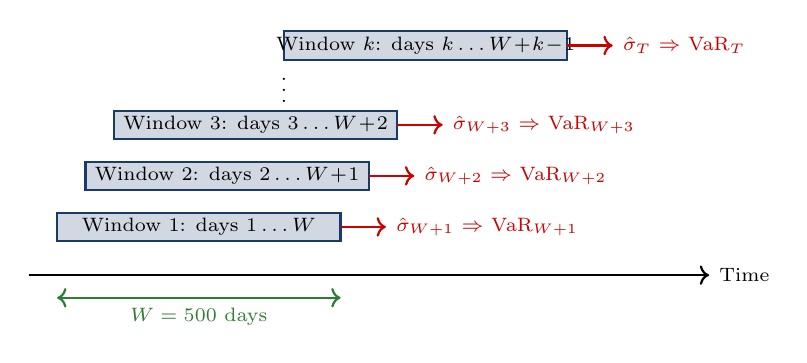
\begin{tikzpicture}[scale=0.72, every node/.style={font=\scriptsize}]
        % Timeline
        \draw[->, thick] (0,0) -- (12,0) node[right] {Time};

        % Window 1
        \draw[fill=MainBlue!20, draw=MainBlue, thick] (0.5,0.6) rectangle (5.5,1.1);
        \node at (3,0.85) {Window 1: days $1 \ldots W$};
        \draw[->, thick, IDAred] (5.5,0.85) -- (6.3,0.85) node[right] {$\hat{\sigma}_{W+1}$ $\Rightarrow$ VaR$_{W+1}$};

        % Window 2
        \draw[fill=MainBlue!20, draw=MainBlue, thick] (1.0,1.5) rectangle (6.0,2.0);
        \node at (3.5,1.75) {Window 2: days $2 \ldots W\!+\!1$};
        \draw[->, thick, IDAred] (6.0,1.75) -- (6.8,1.75) node[right] {$\hat{\sigma}_{W+2}$ $\Rightarrow$ VaR$_{W+2}$};

        % Window 3
        \draw[fill=MainBlue!20, draw=MainBlue, thick] (1.5,2.4) rectangle (6.5,2.9);
        \node at (4,2.65) {Window 3: days $3 \ldots W\!+\!2$};
        \draw[->, thick, IDAred] (6.5,2.65) -- (7.3,2.65) node[right] {$\hat{\sigma}_{W+3}$ $\Rightarrow$ VaR$_{W+3}$};

        % Dots
        \node at (4.5,3.4) {$\vdots$};

        % Window T
        \draw[fill=MainBlue!20, draw=MainBlue, thick] (4.5,3.8) rectangle (9.5,4.3);
        \node at (7,4.05) {Window $k$: days $k \ldots W\!+\!k\!-\!1$};
        \draw[->, thick, IDAred] (9.5,4.05) -- (10.3,4.05) node[right] {$\hat{\sigma}_{T}$ $\Rightarrow$ VaR$_{T}$};

        % Annotations
        \draw[<->, thick, Forest] (0.5,-0.4) -- (5.5,-0.4) node[midway, below] {$W = 500$ days};
    \end{tikzpicture}
    \end{center}
    \vspace{-0.2cm}
    {\small
    \begin{block}{Result}
        \begin{itemize}\setlength{\itemsep}{0pt}
            \item We obtain the series $\{\text{VaR}_{\alpha,t}\}_{t=W+1}^{T}$ $\Rightarrow$ a \textbf{different} threshold every day
            \item VaR adapts to the current regime: increases during volatile periods, decreases during calm ones
            \item Compare $r_t$ with $-\text{VaR}_{\alpha,t}$ to identify violations
        \end{itemize}
    \end{block}
    }
\end{frame}

\begin{frame}{Volatility Forecast with Confidence Intervals}
    \vspace{-0.2cm}
    {\scriptsize
    \begin{cminipage}{0.95\textwidth}
    \vspace{-0.2cm}
    {\footnotesize
    \begin{block}{Interpretation}
        \begin{itemize}\setlength{\itemsep}{0pt}
            \item Forecast converges to $\bar{\sigma}$
            \item Uncertainty increases with forecast horizon
        \end{itemize}
    \end{block}
    }
    \end{cminipage}
    }
    \begin{center}
        \includegraphics[width=0.95\textwidth, height=0.50\textheight, keepaspectratio]{garch_volatility_forecast.pdf}
    \end{center}
    \quantlet{TSA\_ch5\_vol\_ci}{https://github.com/QuantLet/TSA/tree/main/TSA_ch5/TSA_ch5_vol_ci}
\end{frame}

\begin{frame}{Rolling Forecast: Step-by-Step Prediction}
    \vspace{-0.2cm}
    \begin{columns}[T]
        \column{0.55\textwidth}
        {\scriptsize
        \small
        \begin{block}{Procedure}
        {\footnotesize
            S\&P 500, W=500, GARCH(1,1)-t
            \begin{itemize}\setlength{\itemsep}{1pt}
                \item Re-estimate GARCH on $[t\!-\!W,\; t\!-\!1]$; forecast $\hat{\sigma}_{t|t-1}$
                \item Compare with realized vol.\ (20-day rolling std.)
            \end{itemize}
        }
        \end{block}
        \vspace{-0.1cm}
        \begin{exampleblock}{Results (2015 days OOS)}
        {\footnotesize
            \begin{itemize}\setlength{\itemsep}{1pt}
                \item $\rho = 0.938$ $\succ$ excellent tracking; MAE $= 0.15\%$, RMSE $= 0.24\%$
                \item COVID-19: temporary under-prediction, rapid adaptation
            \end{itemize}
        }
        \end{exampleblock}
        }
        \column{0.43\textwidth}
        \vspace{-0.3cm}
        \begin{center}
            \includegraphics[width=\textwidth, keepaspectratio]{garch_rolling_forecast.pdf}
        \end{center}
        \quantlet{TSA\_ch5\_rolling\_forecast}{https://github.com/QuantLet/TSA/tree/main/TSA_ch5/TSA_ch5_rolling_forecast}
    \end{columns}
\end{frame}

%=============================================================================
% SECTION 7: PYTHON IMPLEMENTATION
%=============================================================================
\section{Python Implementation}

\begin{frame}[fragile]{GARCH Estimation in Python: arch Package}
\small
\begin{columns}[T]
\begin{column}{0.55\textwidth}
\begin{block}{Python Code}
\begin{verbatim}
pip install arch
from arch import arch_model

model = arch_model(returns,
    vol='Garch', p=1, q=1,
    dist='normal')
results = model.fit(disp='off')
print(results.summary())
\end{verbatim}
\end{block}
\end{column}
\begin{column}{0.43\textwidth}
\begin{block}{Key Parameters}
\begin{itemize}\setlength{\itemsep}{0pt}
    \item \textbf{vol}: model type
        \begin{itemize}\setlength{\itemsep}{0pt}
            \item \texttt{'Garch'}, \texttt{'EGARCH'}
        \end{itemize}
    \item \textbf{p, q}: GARCH order
        \begin{itemize}\setlength{\itemsep}{0pt}
            \item p=1, q=1 standard
        \end{itemize}
    \item \textbf{dist}: distribution
        \begin{itemize}\setlength{\itemsep}{0pt}
            \item \texttt{'normal'}, \texttt{'t'}
        \end{itemize}
\end{itemize}
\end{block}
\end{column}
\end{columns}
    \quantlet{TSA\_ch5\_garch}{https://github.com/QuantLet/TSA/tree/main/TSA_ch5/TSA_ch5_garch}
\end{frame}

\begin{frame}[fragile]{Asymmetric Models in Python}
\small
\begin{block}{EGARCH and GJR-GARCH}
\begin{verbatim}
# EGARCH
model_egarch = arch_model(returns, vol='EGARCH', p=1, q=1)
# GJR-GARCH (o=1 adds the asymmetric term)
model_gjr = arch_model(returns, vol='Garch', p=1, o=1, q=1)
\end{verbatim}
\end{block}
\vspace{-0.1cm}
\begin{block}{Alternative Distributions}
\begin{verbatim}
# Student-t for fat tails
model_t = arch_model(returns, vol='Garch', p=1, q=1, dist='t')
# Skewed Student-t for asymmetry and fat tails
model_skewt = arch_model(returns, vol='Garch', p=1, q=1,
                         dist='skewt')
\end{verbatim}
\end{block}
    \quantlet{TSA\_ch5\_egarch}{https://github.com/QuantLet/TSA/tree/main/TSA_ch5/TSA_ch5_egarch}
\end{frame}

\begin{frame}[fragile]{Forecasting and Diagnostics}
    \vspace{-0.2cm}
\small
\begin{block}{Volatility Forecast}
\begin{verbatim}
forecasts = results.forecast(horizon=10)
vol_forecast = np.sqrt(forecasts.variance.values[-1,:])
\end{verbatim}
\end{block}
\vspace{-0.1cm}
\begin{block}{Diagnostics and VaR}
\begin{verbatim}
std_resid = results.std_resid
lb_test = acorr_ljungbox(std_resid**2, lags=10)
sigma = np.sqrt(forecasts.variance.values[-1, 0])
VaR_5pct = 1.645 * sigma
\end{verbatim}
\end{block}
    \quantlet{TSA\_ch5\_forecast}{https://github.com/QuantLet/TSA/tree/main/TSA_ch5/TSA_ch5_forecast}
\end{frame}

\begin{frame}{VaR Backtesting: Kupiec Test}
    \begin{block}{Unconditional Coverage Test}
        Tests whether the observed violation rate equals the expected rate $p$ (e.g., 1\% for VaR 1\%).

        \vspace{0.2cm}

        Let $N$ = number of VaR violations, $T$ = total observations, $\hat{p} = N/T$.

        \vspace{0.2cm}

        \textbf{Likelihood Ratio Statistic:}
        \[
            LR_{uc} = -2\ln\left[\frac{(1-p)^{T-N} p^N}{(1-\hat{p})^{T-N} \hat{p}^N}\right] \sim \chi^2(1)
        \]
    \end{block}

    \vspace{0.2cm}

    \begin{alertblock}{Hypotheses}
        \begin{itemize}
            \item $H_0$: $\hat{p} = p$ (VaR model is correctly calibrated)
            \item $H_1$: $\hat{p} \neq p$ (VaR model under- or over-estimates risk)
        \end{itemize}
    \end{alertblock}
\end{frame}

\begin{frame}{VaR Backtesting: Christoffersen Test}
    \begin{cminipage}{0.95\textwidth}
    \vspace{-0.3cm}
    \begin{block}{Conditional Coverage Test}
        Tests both \textbf{unconditional coverage} and \textbf{independence} of violations.

        Violations should be independent --- no clustering of exceptions!
    \end{block}
    \vspace{-0.1cm}
    \begin{block}{Test Components}
        \begin{itemize}\setlength{\itemsep}{0pt}
            \item \textbf{Independence test} ($LR_{ind}$): Tests if violations are serially independent
            \item \textbf{Conditional coverage}: $LR_{cc} = LR_{uc} + LR_{ind} \sim \chi^2(2)$
        \end{itemize}
    \end{block}
    \vspace{-0.1cm}
    \begin{alertblock}{Interpretation}
        Reject $LR_{uc}$: wrong frequency; Reject $LR_{ind}$: clustered violations; Reject $LR_{cc}$: model fails
    \end{alertblock}
    \end{cminipage}
\end{frame}

\begin{frame}[fragile]{VaR Backtesting: Rolling Window Python}
\small
\begin{block}{Rolling VaR Estimation with GARCH(1,1)-t}
{\footnotesize
\begin{verbatim}
from arch import arch_model
import numpy as np
from scipy import stats

returns = ...  # pd.Series with daily returns
window = 500; alpha = 0.01
VaR_series = pd.Series(index=returns.index[window:], dtype=float)

for t in range(window, len(returns)):
    train = returns.iloc[t-window:t]
    model = arch_model(train, vol='Garch', p=1, q=1, dist='t')
    res = model.fit(disp='off', show_warning=False)
    fcast = res.forecast(horizon=1, reindex=False)
    sigma = np.sqrt(fcast.variance.values[-1, 0])
    nu = res.params['nu']   # Student-t degrees of freedom
    q = stats.t.ppf(alpha, nu) * np.sqrt((nu-2)/nu)
    VaR_series.iloc[t - window] = -q * sigma
\end{verbatim}
}
\end{block}
    \quantlet{TSA\_ch5\_backtest\_py}{https://github.com/QuantLet/TSA/tree/main/TSA_ch5/TSA_ch5_backtest_py}
\end{frame}

\begin{frame}[fragile]{VaR Backtesting: Kupiec Test Python}
\small
\begin{block}{Function \texttt{kupiec\_test()}}
{\footnotesize
\begin{verbatim}
def kupiec_test(violations, T, alpha=0.01):
    """Kupiec (1995) unconditional coverage LR test."""
    x = violations.sum()          # observed violations
    p_hat = x / T                 # empirical rate
    if x == 0 or x == T:
        return np.nan, np.nan
    LR_uc = -2 * (x*np.log(alpha) + (T-x)*np.log(1-alpha)
                 - x*np.log(p_hat) - (T-x)*np.log(1-p_hat))
    p_value = 1 - stats.chi2.cdf(LR_uc, df=1)
    return LR_uc, p_value
\end{verbatim}
}
\end{block}
\vspace{-0.2cm}
\begin{exampleblock}{Usage}
{\footnotesize
\begin{verbatim}
violations = returns[window:] < -VaR_series
LR, pval = kupiec_test(violations, len(violations))
print(f"Kupiec LR = {LR:.3f}, p-value = {pval:.4f}")
# p-value < 0.05 => reject H0 => inadequate model
\end{verbatim}
}
\end{exampleblock}
\end{frame}

\begin{frame}[fragile]{VaR Backtesting: Christoffersen Test Python}
\small
\begin{block}{Function \texttt{christoffersen\_test()}}
{\footnotesize
\begin{verbatim}
def christoffersen_test(violations):
    """Christoffersen (1998) conditional coverage test."""
    V = violations.astype(int).values
    # Transition matrix: n_ij
    n00 = ((V[:-1]==0) & (V[1:]==0)).sum()
    n01 = ((V[:-1]==0) & (V[1:]==1)).sum()
    n10 = ((V[:-1]==1) & (V[1:]==0)).sum()
    n11 = ((V[:-1]==1) & (V[1:]==1)).sum()
    # Conditional probabilities
    p01 = n01/(n00+n01) if (n00+n01)>0 else 0
    p11 = n11/(n10+n11) if (n10+n11)>0 else 0
    p = (n01+n11) / (n00+n01+n10+n11)  # global rate
    if p01==0 or p11==0 or p==0 or p==1: return np.nan, np.nan
    LR_ind = -2*(np.log(1-p)*(n00+n10) + np.log(p)*(n01+n11)
        - np.log(1-p01)*n00 - np.log(p01)*n01
        - np.log(1-p11)*n10 - np.log(p11)*n11)
    p_value = 1 - stats.chi2.cdf(LR_ind, df=1)
    return LR_ind, p_value
\end{verbatim}
}
\end{block}
\end{frame}

\begin{frame}[fragile]{Full Backtesting: Results and Decision}
\small
\begin{block}{Application S\&P 500 (T=500, VaR 1\%)}
{\scriptsize
\begin{verbatim}
violations = returns[window:] < -VaR_series
n_viol = violations.sum()
T = len(violations)
rate = n_viol / T
print(f"Violations: {n_viol}/{T} (rate = {rate:.2%})")
LR_uc, p_uc = kupiec_test(violations, T, alpha=0.01)
LR_ind, p_ind = christoffersen_test(violations)
LR_cc = LR_uc + LR_ind   # combined test ~ chi2(2)
p_cc = 1 - stats.chi2.cdf(LR_cc, df=2)
\end{verbatim}
}
\end{block}
\vspace{-0.3cm}
\begin{exampleblock}{Typical Output}
{\scriptsize
\begin{verbatim}
Violations: 13/500 (rate = 2.60%)
Kupiec    LR = 5.83,  p-value = 0.0157  => Rejected (p<0.05)
Independ. LR = 0.42,  p-value = 0.5171  => Accepted
Combined  LR = 6.25,  p-value = 0.0439  => Rejected
Basel Zone: RED (>=10 violations) => Inadequate model
\end{verbatim}
}
\end{exampleblock}
    \quantlet{TSA\_ch5\_backtest\_full}{https://github.com/QuantLet/TSA/tree/main/TSA_ch5/TSA_ch5_backtest_full}
\end{frame}

%=============================================================================
% SECTION 7b: ARMA-GARCH JOINT MODELING
%=============================================================================

\begin{frame}{ARMA-GARCH: Joint Mean and Variance Modeling}
    \begin{cminipage}{0.95\textwidth}
\small
    \begin{block}{Why Joint Modeling?}
        \textbf{Serial correlation} $\Rightarrow$ ARMA for mean; \textbf{Volatility clustering} $\Rightarrow$ GARCH for variance.
    \end{block}
    \vspace{-0.1cm}
    \begin{defn}[ARMA(p,q)-GARCH(r,s)]
        \textbf{Mean equation}: $r_t = \mu + \sum_{i=1}^{p} \phi_i (r_{t-i} - \mu) + \sum_{j=1}^{q} \theta_j \varepsilon_{t-j} + \varepsilon_t$

        \textbf{Variance equation}: $\varepsilon_t = \sigma_t z_t$, \quad $\sigma_t^2 = \omega + \sum_{i=1}^{r} \alpha_i \varepsilon_{t-i}^2 + \sum_{j=1}^{s} \beta_j \sigma_{t-j}^2$
    \end{defn}
    \end{cminipage}
\end{frame}

\begin{frame}{ARMA-GARCH: Model Selection Strategy}
    \begin{cminipage}{0.95\textwidth}
    \small
    \begin{block}{Step-by-Step Approach}
        \begin{enumerate}\setlength{\itemsep}{0pt}
            \item \textbf{Identify mean model}: Check ACF/PACF of returns for ARMA structure
            \item \textbf{Test for ARCH effects}: Apply ARCH-LM test to residuals
            \item \textbf{Specify variance model}: Usually GARCH(1,1) is sufficient
            \item \textbf{Joint estimation}: Estimate both equations via MLE
            \item \textbf{Diagnostic checking}: Standardized residuals should be i.i.d.
        \end{enumerate}
    \end{block}

    \vspace{0.2cm}

    \begin{alertblock}{Common Specifications}
        \begin{itemize}\setlength{\itemsep}{0pt}
            \item \textbf{Stock returns}: AR(1)-GARCH(1,1) or ARMA(1,1)-GARCH(1,1)
            \item \textbf{Exchange rates}: Often just GARCH(1,1) (no mean dynamics)
            \item \textbf{Interest rates}: AR(1)-EGARCH(1,1) for leverage effects
        \end{itemize}
    \end{alertblock}
    \end{cminipage}
\end{frame}

\begin{frame}[fragile]{ARMA-GARCH: Python Implementation}
\begin{block}{Using the \texttt{arch} Package}
\begin{verbatim}
from arch import arch_model
model = arch_model(returns,
                   mean='ARX',
                   lags=1,
                   vol='Garch',
                   p=1, q=1,
                   dist='t')
result = model.fit(disp='off')
print(result.summary())
\end{verbatim}
\end{block}
\begin{exampleblock}{Parameters}
\texttt{mean='ARX'}: ARMA mean; \texttt{lags=1}: AR(1); \texttt{dist='t'}: Student-t
\end{exampleblock}
    \quantlet{TSA\_ch5\_armagarch}{https://github.com/QuantLet/TSA/tree/main/TSA_ch5/TSA_ch5_armagarch}
\end{frame}

\begin{frame}[fragile]{ARMA-GARCH: Complete Example}
\begin{verbatim}
from arch import arch_model
model = arch_model(returns,
                   mean='ARX', lags=[1],
                   vol='EGARCH', p=1, q=1,
                   dist='skewt')
result = model.fit(update_freq=0)
cond_mean = result.conditional_mean
cond_vol = result.conditional_volatility
forecasts = result.forecast(horizon=5)
\end{verbatim}
\begin{exampleblock}{Note}
For MA terms, use \texttt{mean='HARX'} or pre-filter with statsmodels ARIMA.
\end{exampleblock}
\end{frame}

%=============================================================================
% SECTION 8: CASE STUDY
%=============================================================================
\section{Case Study: S\&P 500}

\begin{frame}{Step 1: Data --- S\&P 500 Daily Returns}
    \vspace{-0.2cm}
    \begin{columns}[T]
        \column{0.55\textwidth}
        {\scriptsize
        \begin{cminipage}{0.95\textwidth}
        \vspace{-0.3cm}
        {\small
        \begin{block}{Data Description}
            \begin{itemize}\setlength{\itemsep}{0pt}
                \item \textbf{Source}: Yahoo Finance, S\&P 500, daily data 2000--2024 ($T > 6000$)
                \item \textbf{Returns}: $r_t = \ln(P_t/P_{t-1}) \times 100$
            \end{itemize}
        \end{block}
        \vspace{-0.2cm}
        \begin{exampleblock}{Descriptive Statistics}
            \vspace{-0.1cm}
            \begin{center}
            {\footnotesize
            \begin{tabular}{cccccc}
                \toprule
                Mean & Std. Dev. & Skewness & Kurtosis & Min & Max \\
                \midrule
                0.034\% & 1.21\% & $-0.29$ & 13.8 & $-12.8\%$ & $+11.0\%$ \\
                \bottomrule
            \end{tabular}
            }
            \end{center}
            \vspace{-0.1cm}
            \begin{itemize}\setlength{\itemsep}{0pt}
                \item Fat tails (kurtosis $\gg 3$) and negative skewness $\Rightarrow$ ARCH effects
            \end{itemize}
        \end{exampleblock}
        }
        \end{cminipage}
        }
        \column{0.43\textwidth}
        \vspace{-0.3cm}
        \begin{center}
            \includegraphics[width=\textwidth, keepaspectratio]{garch_sp500_returns.pdf}
        \end{center}
        \quantlet{TSA\_ch5\_sp500}{https://github.com/QuantLet/TSA/tree/main/TSA_ch5/TSA_ch5_sp500}
    \end{columns}
\end{frame}

\begin{frame}[fragile]{Step 2: Testing for ARCH Effects}
    \small
    \begin{block}{Python Code --- ARCH-LM and Ljung-Box on $r_t^2$}
        {\scriptsize
\begin{verbatim}
import yfinance as yf
from statsmodels.stats.diagnostic import het_arch, acorr_ljungbox
sp = yf.download('^GSPC', start='2000-01-01', end='2024-12-31')
returns = np.log(sp['Close']).diff().dropna() * 100
# ARCH-LM test (Engle, 1982)
lm_stat, lm_pval, _, _ = het_arch(returns, nlags=10)
# Ljung-Box on squared returns
lb = acorr_ljungbox(returns**2, lags=20)
\end{verbatim}
        }
    \end{block}
    \vspace{-0.3cm}
    \begin{exampleblock}{Results}
        {\small
        \begin{tabular}{lcc}
            \toprule
            \textbf{Test} & \textbf{Statistic} & \textbf{p-value} \\
            \midrule
            ARCH-LM (10 lags) & 892.4 & $< 0.0001$ \\
            Ljung-Box $r_t^2$ (lag 20) & 4217.6 & $< 0.0001$ \\
            \bottomrule
        \end{tabular}
        }
        \begin{itemize}\setlength{\itemsep}{0pt}
            \item \textbf{Conclusion}: Strong ARCH effects $\Rightarrow$ significant heteroskedasticity
        \end{itemize}
    \end{exampleblock}
\end{frame}

\begin{frame}{Step 3: Estimated Parameters --- Comparison}
    \vspace{-0.2cm}
    \begin{columns}[T]
        \column{0.55\textwidth}
        {\scriptsize
        \begin{cminipage}{0.95\textwidth}
        \vspace{-0.3cm}
        \vspace{-0.3cm}
        {\scriptsize
        \begin{block}{Estimated Parameters Table}
            \begin{center}
            \begin{tabular}{lccccccc}
                \toprule
                \textbf{Model} & $\omega$ & $\alpha$ & $\beta$ & $\gamma$ & $\alpha\!+\!\beta$ & $\nu$ & \textbf{HL} \\
                \midrule
                GARCH-N & 0.011 & 0.088 & 0.901 & --- & 0.989 & --- & 60 days \\
                GARCH-t & 0.011 & 0.088 & 0.900 & --- & 0.989 & 6.42 & 60 days \\
                EGARCH-t & 0.003 & 0.103 & 0.987 & $-$0.120 & --- & 6.38 & --- \\
                GJR-t & 0.010 & 0.022 & 0.906 & 0.126 & 0.991 & 6.51 & 78 days \\
                \bottomrule
            \end{tabular}
            \end{center}
        \end{block}
        \vspace{-0.1cm}
        \begin{alertblock}{Interpretation}
            \begin{itemize}\setlength{\itemsep}{0pt}
                \item EGARCH $\gamma = -0.12$ \textbf{significant} $\Rightarrow$ \textbf{leverage effect confirmed}
                \item GJR: $\alpha_{\text{neg}} = \alpha + \gamma = 0.148$ vs $\alpha_{\text{pos}} = 0.022$ $\Rightarrow$ strong asymmetry
            \end{itemize}
        \end{alertblock}
        }
        \end{cminipage}
        }
        \column{0.43\textwidth}
        \vspace{-0.3cm}
        \begin{center}
            \includegraphics[width=\textwidth, keepaspectratio]{garch_sp500_volatility.pdf}
        \end{center}
        \quantlet{TSA\_ch5\_sp500\_garch}{https://github.com/QuantLet/TSA/tree/main/TSA_ch5/TSA_ch5_sp500_garch}
    \end{columns}
\end{frame}

\begin{frame}[fragile]{Step 3: Estimating Multiple GARCH Models}
\begin{block}{Python Code --- Estimating 4 candidate models}
{\scriptsize
\begin{verbatim}
from arch import arch_model
models = {}
m1 = arch_model(returns, vol='Garch', p=1, q=1, dist='normal')
models['GARCH-N'] = m1.fit(disp='off')
m2 = arch_model(returns, vol='Garch', p=1, q=1, dist='t')
models['GARCH-t'] = m2.fit(disp='off')
m3 = arch_model(returns, vol='EGARCH', p=1, q=1, dist='t')
models['EGARCH-t'] = m3.fit(disp='off')
m4 = arch_model(returns, vol='GARCH', p=1, o=1, q=1, dist='t')
models['GJR-t'] = m4.fit(disp='off')
\end{verbatim}
}
\end{block}
\vspace{-0.2cm}
{\footnotesize
\begin{alertblock}{Strategy}
    \begin{itemize}\setlength{\itemsep}{0pt}
        \item Estimate symmetric \textbf{and} asymmetric models, with different distributions
        \item Final choice: \textbf{AIC/BIC} + \textbf{diagnostics} + \textbf{economic interpretation}
    \end{itemize}
\end{alertblock}
}
\end{frame}

\begin{frame}{Step 5: Leverage Effect --- Visualization}
    \vspace{-0.2cm}
    \begin{columns}[T]
        \column{0.55\textwidth}
        {\scriptsize
        \begin{block}{GARCH vs EGARCH --- Volatility Differences}
            \begin{itemize}\setlength{\itemsep}{0pt}
                \item EGARCH produces \textbf{higher} volatility after negative shocks (2008, 2020)
                \item Symmetric GARCH \textbf{underestimates} risk during crisis periods
                \item Difference: up to 2--3 percentage points in daily volatility
            \end{itemize}
        \end{block}
        }
        \column{0.43\textwidth}
        \vspace{-0.3cm}
        \begin{center}
            \includegraphics[width=\textwidth, keepaspectratio]{garch_sp500_comparison.pdf}
        \end{center}
        \quantlet{TSA\_ch5\_sp500\_comp}{https://github.com/QuantLet/TSA/tree/main/TSA_ch5/TSA_ch5_sp500_comp}
    \end{columns}
\end{frame}

\begin{frame}{Step 4: Model Selection --- AIC/BIC}
    \begin{cminipage}{0.95\textwidth}
    \begin{block}{Information Criteria}
        \begin{center}
        {\small
        \begin{tabular}{lcccl}
            \toprule
            \textbf{Model} & \textbf{Log-Lik} & \textbf{AIC} & \textbf{BIC} & \textbf{Rank} \\
            \midrule
            GARCH(1,1)-N & $-$8042.3 & 16090.6 & 16111.0 & 4 \\
            GARCH(1,1)-t & $-$7981.5 & 15971.0 & 15997.8 & 3 \\
            EGARCH(1,1)-t & $-$7964.2 & \textbf{15938.4} & \textbf{15971.6} & \textbf{1} \\
            GJR-GARCH(1,1)-t & $-$7968.1 & 15946.2 & 15979.4 & 2 \\
            \bottomrule
        \end{tabular}
        }
        \end{center}
    \end{block}
    \begin{exampleblock}{Decision}
        \begin{itemize}\setlength{\itemsep}{0pt}
            \item \textbf{EGARCH(1,1)-t wins}: lowest AIC \textbf{and} BIC
            \item Student-t superior to Normal ($\Delta$AIC $\approx 120$) $\Rightarrow$ fat tails matter!
            \item Leverage effect justifies asymmetric models ($\Delta$AIC $\approx 33$ vs GARCH-t)
        \end{itemize}
    \end{exampleblock}
    \end{cminipage}
\end{frame}

\begin{frame}{Step 5: Diagnostics --- EGARCH(1,1)-t}
    \vspace{-0.2cm}
    \begin{columns}[T]
        \column{0.55\textwidth}
        {\scriptsize
        \begin{block}{Checks on Standardized Residuals $z_t = \varepsilon_t / \hat{\sigma}_t$}
            \begin{itemize}\setlength{\itemsep}{0pt}
                \item \textbf{Ljung-Box} on $z_t$: p-value $= 0.38$ --- no residual autocorrelation
                \item \textbf{Ljung-Box} on $z_t^2$: p-value $= 0.52$ --- \textbf{ARCH effects eliminated}
                \item \textbf{Q-Q plot}: points follow the theoretical Student-t line
                \item \textbf{Conclusion}: EGARCH(1,1)-t adequately captures volatility dynamics
            \end{itemize}
        \end{block}
        }
        \column{0.43\textwidth}
        \vspace{-0.3cm}
        \begin{center}
            \includegraphics[width=\textwidth, keepaspectratio]{garch_diagnostics.pdf}
        \end{center}
        \quantlet{TSA\_ch5\_sp500\_diag}{https://github.com/QuantLet/TSA/tree/main/TSA_ch5/TSA_ch5_sp500_diag}
    \end{columns}
\end{frame}

\begin{frame}{Step 6: Backtesting Rolling VaR --- S\&P 500}
    \vspace{-0.2cm}
    \begin{columns}[T]
        \column{0.55\textwidth}
        {\scriptsize
        \begin{cminipage}{0.95\textwidth}
        \vspace{-0.3cm}
        \vspace{-0.3cm}
        {\small
        \begin{exampleblock}{Kupiec + Christoffersen Results (2015 days out-of-sample)}
            \vspace{-0.1cm}
            \begin{center}
            {\footnotesize
            \begin{tabular}{lccl}
                \toprule
                \textbf{Test} & \textbf{Statistic} & \textbf{p-value} & \textbf{Decision} \\
                \midrule
                Violations & 27/2015 ($\hat{p}=1.34\%$) & --- & \textcolor{Forest}{\textbf{Green}} zone \\
                Kupiec (uc) & 2.13 & 0.145 & \textcolor{Forest}{Accepted} \\
                Christoffersen (ind) & 0.79 & 0.375 & \textcolor{Forest}{Accepted} \\
                Combined (cc) & 2.91 & 0.233 & \textcolor{Forest}{Accepted} \\
                \bottomrule
            \end{tabular}
            }
            \end{center}
        \end{exampleblock}
        }
        \end{cminipage}
        }
        \column{0.43\textwidth}
        \vspace{-0.3cm}
        \begin{center}
            \includegraphics[width=\textwidth, keepaspectratio]{garch_sp500_rolling_var.pdf}
        \end{center}
        \quantlet{TSA\_ch5\_sp500\_var}{https://github.com/QuantLet/TSA/tree/main/TSA_ch5/TSA_ch5_sp500_var}
    \end{columns}
\end{frame}

\begin{frame}[fragile]{Step 6: VaR Rolling Window --- S\&P 500}
    \small
    \begin{block}{Rolling Window Procedure (W=500 days, VaR 1\%)}
        {\scriptsize
\begin{verbatim}
from scipy import stats
W = 500; alpha = 0.01
VaR_roll = pd.Series(index=returns.index[W:], dtype=float)
for t in range(W, len(returns)):
    train = returns.iloc[t-W:t]
    m = arch_model(train, vol='Garch', p=1, q=1, dist='t')
    res = m.fit(disp='off', show_warning=False)
    fcast = res.forecast(horizon=1, reindex=False)
    sigma = np.sqrt(fcast.variance.values[-1, 0])
    nu = res.params['nu']
    VaR_roll.iloc[t-W] = -stats.t.ppf(alpha,nu)*np.sqrt((nu-2)/nu)*sigma
\end{verbatim}
        }
    \end{block}
    \vspace{-0.3cm}
    {\small
    \begin{exampleblock}{Rolling VaR Characteristics S\&P 500 (2017--2024)}
        \begin{itemize}\setlength{\itemsep}{0pt}
            \item Mean VaR: 2.53\% ($\approx$ EUR 253,000 / 10M EUR)
            \item Max VaR: 22.02\% $\Rightarrow$ COVID-19 crisis ($\approx$ EUR 2,202,000)
            \item Min VaR: 0.91\% $\Rightarrow$ calm period ($\approx$ EUR 91,000)
            \item \textbf{VaR adapts}: automatically increases during crisis periods
        \end{itemize}
    \end{exampleblock}
    }
\end{frame}

\begin{frame}{Step 7: Conclusions --- S\&P 500 Case Study}
    \begin{cminipage}{0.95\textwidth}
    \begin{block}{Step-by-Step Methodology Summary}
        \begin{enumerate}\setlength{\itemsep}{2pt}
            \item \textbf{Data}: log returns, descriptive statistics $\Rightarrow$ fat tails, skewness
            \item \textbf{ARCH test}: ARCH-LM + Ljung-Box on $r_t^2$ $\Rightarrow$ significant ARCH effects
            \item \textbf{Estimation}: 4 candidate models (symmetric/asymmetric $\times$ Normal/Student-t)
            \item \textbf{Selection}: AIC/BIC $\Rightarrow$ \textbf{EGARCH(1,1)-t} winner
            \item \textbf{Diagnostics}: standardized residuals $\Rightarrow$ model adequate
            \item \textbf{VaR}: rolling window + Kupiec/Christoffersen backtesting $\Rightarrow$ model \textbf{validated}
        \end{enumerate}
    \end{block}
    \vspace{0.1cm}
    \begin{alertblock}{Key Lessons}
        \begin{itemize}\setlength{\itemsep}{0pt}
            \item Student-t distribution is \textbf{essential} for financial data
            \item Leverage effect: asymmetric models \textbf{mandatory} for equities
            \item Systematic backtesting: not just ``looks good'', but \textbf{statistically tested}
        \end{itemize}
    \end{alertblock}
    \end{cminipage}
\end{frame}

%=============================================================================
% SECTION 9: CASE STUDY --- Bitcoin
%=============================================================================
\section{Case Study: Bitcoin}

\begin{frame}{Step 1: Data --- Bitcoin Daily Returns}
    \vspace{-0.2cm}
    \begin{columns}[T]
        \column{0.55\textwidth}
        {\scriptsize
        \begin{cminipage}{0.95\textwidth}
        \vspace{-0.3cm}
        \vspace{-0.35cm}
        {\footnotesize
        \begin{block}{Data Description}
            \begin{itemize}\setlength{\itemsep}{0pt}
                \item \textbf{Source}: Yahoo Finance (BTC-USD), daily data 2018--2024
                \item Log returns: mean $\approx 0.05\%$, volatility $\approx 3.5\%$
            \end{itemize}
        \end{block}
        \vspace{-0.2cm}
        \begin{exampleblock}{Descriptive Statistics}
            \vspace{-0.1cm}
            \begin{center}
            {\footnotesize
            \begin{tabular}{cccccc}
                \toprule
                Mean & Std. Dev. & Skewness & Kurtosis & Min & Max \\
                \midrule
                0.05\% & 3.48\% & $-0.72$ & 12.1 & $-46.5\%$ & $+22.5\%$ \\
                \bottomrule
            \end{tabular}
            }
            \end{center}
            \vspace{-0.15cm}
            \begin{itemize}\setlength{\itemsep}{0pt}
                \item Volatility $\sim$3$\times$ higher than S\&P 500
                \item Extreme kurtosis --- high risk of large losses
            \end{itemize}
        \end{exampleblock}
        }
        \end{cminipage}
        }
        \column{0.43\textwidth}
        \vspace{-0.3cm}
        \begin{center}
            \includegraphics[width=\textwidth, keepaspectratio]{btc_returns.pdf}
        \end{center}
        \quantlet{TSA\_ch5\_btc}{https://github.com/QuantLet/TSA/tree/main/TSA_ch5/TSA_ch5_btc}
    \end{columns}
\end{frame}

\begin{frame}{Step 2: Testing for ARCH Effects --- Bitcoin}
    \vspace{-0.2cm}
    {\scriptsize
    }
    \begin{center}
        \includegraphics[width=0.95\textwidth, height=0.50\textheight, keepaspectratio]{btc_squared_returns.pdf}
    \end{center}
    \quantlet{TSA\_ch5\_btc\_arch}{https://github.com/QuantLet/TSA/tree/main/TSA_ch5/TSA_ch5_btc_arch}
\end{frame}

\begin{frame}{Step 5: Conditional Volatility --- Bitcoin}
    \vspace{-0.2cm}
    \begin{columns}[T]
        \column{0.55\textwidth}
        {\scriptsize
        \begin{block}{GJR-GARCH(1,1)-t Diagnostics}
            \begin{itemize}\setlength{\itemsep}{0pt}
                \item Ljung-Box on $z_t^2$: p-value $= 0.41$ --- \textbf{ARCH effects eliminated}
                \item Volatility peaks: March 2020 (COVID), May 2022 (Terra/Luna)
                \item Daily volatility: from 1\% (calm periods) to $>$15\% (crises)
            \end{itemize}
        \end{block}
        }
        \column{0.43\textwidth}
        \vspace{-0.3cm}
        \begin{center}
            \includegraphics[width=\textwidth, keepaspectratio]{ch10_bitcoin_garch.pdf}
        \end{center}
        \quantlet{TSA\_ch5\_btc\_garch}{https://github.com/QuantLet/TSA/tree/main/TSA_ch5/TSA_ch5_btc_garch}
    \end{columns}
\end{frame}

\begin{frame}{Steps 3--4: Estimation and Model Selection --- Bitcoin}
    \begin{cminipage}{0.95\textwidth}
    \begin{block}{Estimated Parameters}
        \begin{center}
        {\small
        \begin{tabular}{lccccccc}
            \toprule
            \textbf{Model} & $\omega$ & $\alpha$ & $\beta$ & $\gamma$ & $\alpha\!+\!\beta$ & $\nu$ & \textbf{AIC} \\
            \midrule
            GARCH-t & 0.42 & 0.131 & 0.848 & --- & 0.979 & 4.82 & 9284 \\
            EGARCH-t & 0.08 & 0.184 & 0.976 & $-$0.061 & --- & 4.79 & 9276 \\
            GJR-t & 0.40 & 0.088 & 0.854 & 0.078 & 0.976 & 4.85 & \textbf{9271} \\
            \bottomrule
        \end{tabular}
        }
        \end{center}
    \end{block}
    \begin{block}{Interpretation}
        \begin{itemize}\setlength{\itemsep}{0pt}
            \item \textbf{GJR-GARCH-t wins} (lowest AIC)
            \item $\nu \approx 4.8$: \textbf{much heavier tails} than S\&P 500 ($\nu = 6.4$)
            \item $\alpha = 0.131$ (BTC) vs $0.088$ (S\&P) --- Bitcoin reacts faster to news
            \item Leverage effect weaker than for stocks ($\gamma_{\text{BTC}} = 0.078$ vs $0.126$)
        \end{itemize}
    \end{block}
    \end{cminipage}
\end{frame}

\begin{frame}{Step 6: Backtesting Rolling VaR --- Bitcoin}
    \vspace{-0.2cm}
    \begin{columns}[T]
        \column{0.55\textwidth}
        {\scriptsize
        \begin{cminipage}{0.95\textwidth}
        \vspace{-0.4cm}
        \vspace{-0.35cm}
        {\scriptsize
        \begin{block}{Statistical Tests (2421 days out-of-sample)}
            \vspace{-0.15cm}
            \begin{center}
            \begin{tabular}{lccl}
                \toprule
                \textbf{Test} & \textbf{Statistic} & \textbf{p-value} & \textbf{Decision} \\
                \midrule
                Violations & 28/2421 ($\hat{p}=1.16\%$) & --- & \textcolor{Forest}{\textbf{Green}} zone \\
                Kupiec (uc) & 0.57 & 0.450 & \textcolor{Forest}{Accepted} \\
                Christoffersen (ind) & 0.94 & 0.333 & \textcolor{Forest}{Accepted} \\
                Combined (cc) & 1.51 & 0.471 & \textcolor{Forest}{Accepted} \\
                \bottomrule
            \end{tabular}
            \end{center}
            \vspace{-0.15cm}
        \end{block}
        \vspace{-0.15cm}
        \begin{alertblock}{Interpretation}
            \begin{itemize}\setlength{\itemsep}{0pt}
                \item Volatility ranges from 3\% to 38\% --- rolling window is \textbf{essential}
                \item All tests \textbf{accepted}: model valid for risk management
            \end{itemize}
        \end{alertblock}
        }
        \end{cminipage}
        }
        \column{0.43\textwidth}
        \vspace{-0.3cm}
        \begin{center}
            \includegraphics[width=\textwidth, keepaspectratio]{garch_btc_rolling_var.pdf}
        \end{center}
        \quantlet{TSA\_ch5\_btc\_var}{https://github.com/QuantLet/TSA/tree/main/TSA_ch5/TSA_ch5_btc_var}
    \end{columns}
\end{frame}

\begin{frame}[fragile]{Step 6: VaR Rolling Window --- Bitcoin}
    \small
    \begin{block}{Rolling Window GJR-GARCH-t (W=500 days, VaR 1\%)}
        {\scriptsize
\begin{verbatim}
W = 500; alpha = 0.01
VaR_btc = pd.Series(index=btc_returns.index[W:], dtype=float)
for t in range(W, len(btc_returns)):
    train = btc_returns.iloc[t-W:t]
    m = arch_model(train, vol='GARCH', p=1, o=1, q=1, dist='t')
    res = m.fit(disp='off', show_warning=False)
    fcast = res.forecast(horizon=1, reindex=False)
    sigma = np.sqrt(fcast.variance.values[-1, 0])
    nu = res.params['nu']
    VaR_btc.iloc[t-W] = -stats.t.ppf(alpha,nu)*np.sqrt((nu-2)/nu)*sigma
\end{verbatim}
        }
    \end{block}
    \vspace{-0.3cm}
    {\small
    \begin{exampleblock}{Rolling VaR Characteristics Bitcoin (2018--2024)}
        \begin{itemize}\setlength{\itemsep}{0pt}
            \item Mean VaR: 9.34\% ($\approx$ EUR 93,400 / 1M EUR)
            \item Max VaR: 37.54\% $\Rightarrow$ COVID crash March 2020
            \item Min VaR: 2.90\% $\Rightarrow$ calm period
            \item Bitcoin: rolling VaR $\sim$4$\times$ larger than S\&P 500 at same exposure
        \end{itemize}
    \end{exampleblock}
    }
\end{frame}

\begin{frame}{Final Comparison: S\&P 500 vs Bitcoin}
    \begin{cminipage}{0.95\textwidth}
    \vspace{-0.3cm}
    {\small
    \begin{block}{Comparative Summary}
        \vspace{-0.1cm}
        \begin{center}
        {\footnotesize
        \begin{tabular}{lcc}
            \toprule
            & \textbf{S\&P 500} & \textbf{Bitcoin} \\
            \midrule
            Average volatility & 1.2\% & 3.5\% \\
            Kurtosis & 13.8 & 12.1 \\
            Student-t $\nu$ & 6.42 & 4.82 \\
            Best model & EGARCH(1,1)-t & GJR-GARCH(1,1)-t \\
            Leverage effect & Strong ($\gamma = -0.12$) & Moderate ($\gamma = 0.078$) \\
            Half-life & $\sim$60 days & $\sim$42 days \\
            Rolling VaR 1\% mean & 2.53\% & 9.34\% \\
            Rolling VaR 1\% max & 22.02\% (COVID) & 37.54\% (COVID) \\
            Kupiec & \textcolor{Forest}{\textbf{Accepted}} (p=0.145) & \textcolor{Forest}{\textbf{Accepted}} (p=0.450) \\
            Christoffersen (ind) & \textcolor{Forest}{\textbf{Accepted}} (p=0.375) & \textcolor{Forest}{\textbf{Accepted}} (p=0.333) \\
            \bottomrule
        \end{tabular}
        }
        \end{center}
    \end{block}
    \vspace{-0.1cm}
    \begin{alertblock}{General Conclusion}
        \begin{itemize}\setlength{\itemsep}{0pt}
            \item Re-estimating GARCH at each step: Kupiec + Christoffersen \textbf{accepted}
            \item Rolling window VaR: \textbf{mandatory} --- static VaR is completely inadequate
            \item Student-t + asymmetric model: \textbf{essential} for both markets
        \end{itemize}
    \end{alertblock}
    }
    \end{cminipage}
\end{frame}

%=============================================================================
% KEY FORMULAS
%=============================================================================
\begin{frame}{Key Formulas}
    \begin{cminipage}{0.95\textwidth}
    \small
    \begin{block}{Volatility Models}
        \begin{itemize}\setlength{\itemsep}{0pt}
            \item \textbf{ARCH(q):} $\sigma_t^2 = \omega + \sum_{i=1}^{q} \alpha_i \varepsilon_{t-i}^2$
            \item \textbf{GARCH(1,1):} $\sigma_t^2 = \omega + \alpha \varepsilon_{t-1}^2 + \beta \sigma_{t-1}^2$
            \item \textbf{EGARCH:} $\ln(\sigma_t^2) = \omega + \alpha(|z_{t-1}| - \E[|z|]) + \gamma z_{t-1} + \beta \ln(\sigma_{t-1}^2)$
            \item \textbf{GJR-GARCH:} $\sigma_t^2 = \omega + \alpha \varepsilon_{t-1}^2 + \gamma \varepsilon_{t-1}^2 I_{t-1} + \beta \sigma_{t-1}^2$
        \end{itemize}
    \end{block}

    \begin{block}{Properties and Measures}
        \begin{itemize}\setlength{\itemsep}{0pt}
            \item \textbf{Unconditional variance:} $\bar{\sigma}^2 = \frac{\omega}{1-\alpha-\beta}$ \quad \textbf{Half-life:} $HL = \frac{\ln(0.5)}{\ln(\alpha+\beta)}$
            \item \textbf{VaR:} $\text{VaR}_\alpha = z_\alpha \cdot \sigma_{T+1}$ \quad \textbf{Stationarity:} $\alpha + \beta < 1$
            \item \textbf{ARCH-LM:} $LM = T \cdot R^2 \sim \chi^2(q)$
        \end{itemize}
    \end{block}
    \end{cminipage}
\end{frame}

%=============================================================================
\section{AI Use Case}
%=============================================================================

\begin{frame}{AI Exercise: Critical Thinking}
    \begin{cminipage}{0.95\textwidth}
    \vspace{-3mm}
    \begin{block}{\footnotesize Prompt to test in ChatGPT / Claude / Copilot}
        {\footnotesize
        ``Download daily S\&P 500 returns using yfinance. Test for ARCH effects, fit a GARCH model, and forecast volatility for the next 20 trading days. Give me complete Python code.''
        }
    \end{block}
    \vspace{-2mm}
    {\footnotesize
    \textbf{Exercise}:
    \begin{enumerate}\setlength{\itemsep}{0pt}
        \item Run the prompt in an LLM of your choice and critically analyze the response.
        \item Does it compute log returns correctly? Does it remove the mean before fitting GARCH?
        \item How does it test for ARCH effects? Does it use Engle's LM test?
        \item Does it separate the mean equation from the variance equation?
        \item Does it discuss asymmetric effects (GJR-GARCH, EGARCH)? Are VaR estimates computed from the conditional distribution?
    \end{enumerate}
    }
    \vspace{-2mm}
    \begin{alertblock}{}
        {\footnotesize \textbf{Warning}: AI-generated code may run without errors and look professional. \textit{That does not mean it is correct.}}
    \end{alertblock}
    \end{cminipage}
\end{frame}

%=============================================================================
% SUMMARY
%=============================================================================
\section{Summary}

\begin{frame}{Summary $\rightarrow$ Chapter 5: Volatility Models}
\small
    \vspace{-0.2cm}
    \begin{cminipage}{0.95\textwidth}
    \begin{block}{Key Concepts}
        \begin{itemize}\setlength{\itemsep}{0pt}
            \item \textbf{ARCH(q)}: conditional variance depends on past squared errors (Nobel 2003)
            \item \textbf{GARCH(p,q)}: adds variance lags for persistence (GARCH(1,1) in 90\% of cases)
            \item \textbf{EGARCH}: allows leverage effect, no positivity constraints
            \item \textbf{GJR-GARCH/TGARCH}: captures asymmetry with indicator variables
        \end{itemize}
    \end{block}
    \vspace{-0.2cm}
    \begin{block}{Applications}
        \begin{itemize}\setlength{\itemsep}{0pt}
            \item Risk measurement and forecasting (VaR, ES)
            \item Derivative pricing, dynamic hedging, portfolio management
        \end{itemize}
    \end{block}
    \vspace{-0.2cm}
    \begin{alertblock}{Practical Tip}
        \begin{itemize}\setlength{\itemsep}{0pt}
            \item Start with GARCH(1,1), check for leverage, choose distribution minimizing AIC/BIC!
                \begin{itemize}\setlength{\itemsep}{0pt}
                    \item Student-t often superior to normal distribution
                \end{itemize}
        \end{itemize}
    \end{alertblock}
    \end{cminipage}
\end{frame}

%=============================================================================
% QUIZ
%=============================================================================
\section{Quiz}

\begin{frame}{Quiz Question 1}
    \begin{cminipage}{0.95\textwidth}
    \begin{alertblock}{Question}
        What best describes the phenomenon of \textit{volatility clustering} in financial series?
    \end{alertblock}

    \vspace{0.3cm}

    \begin{enumerate}[(A)]
        \item Financial returns are normally distributed and independent
        \item Periods of high volatility are followed by high volatility, and vice versa
        \item Volatility is constant over time (homoscedasticity)
        \item Correlation between returns is always positive
    \end{enumerate}
    \end{cminipage}
\end{frame}

\begin{frame}{Quiz Question 1: Answer}
    \begin{cminipage}{0.95\textwidth}
    \begin{exampleblock}{Correct Answer: (B) Periods of high volatility are followed by similar periods}
        Volatility clustering is a fundamental stylized fact of financial series. It implies that conditional variance is \textbf{predictable}, motivating ARCH/GARCH models.
    \end{exampleblock}
    \vspace{0.1cm}
    \begin{center}
        \includegraphics[width=0.95\textwidth, height=0.51\textheight, keepaspectratio]{garch_quiz1_volatility_clustering.pdf}
    \end{center}
    \quantlet{TSA\_ch5\_quiz1\_volatility\_clustering}{https://github.com/QuantLet/TSA/tree/main/TSA_ch5/TSA_ch5_quiz1_volatility_clustering}
    \end{cminipage}
\end{frame}

\begin{frame}{Quiz Question 2}
    \begin{cminipage}{0.95\textwidth}
    \begin{alertblock}{Question}
        What is the main difference between an ARCH(q) and a GARCH(p,q) model?
    \end{alertblock}

    \vspace{0.3cm}

    \begin{enumerate}[(A)]
        \item GARCH models the conditional mean, ARCH models the variance
        \item ARCH includes lags of conditional variance, GARCH does not
        \item GARCH adds lags of conditional variance ($\sigma_{t-j}^2$) beyond squared errors
        \item ARCH is more parsimonious than GARCH
    \end{enumerate}
    \end{cminipage}
\end{frame}

\begin{frame}{Quiz Question 2: Answer}
    \begin{cminipage}{0.95\textwidth}
    \begin{exampleblock}{Correct Answer: (C) GARCH adds lags of conditional variance}
        GARCH(1,1) captures the same persistence as ARCH(q) with only 2 parameters instead of $q$. In practice, GARCH(1,1) is sufficient in 90\% of cases.
    \end{exampleblock}
    \vspace{0.1cm}
    \begin{center}
        \includegraphics[width=0.95\textwidth, height=0.51\textheight, keepaspectratio]{garch_quiz2_arch_vs_garch.pdf}
    \end{center}
    \quantlet{TSA\_ch5\_quiz2\_arch\_vs\_garch}{https://github.com/QuantLet/TSA/tree/main/TSA_ch5/TSA_ch5_quiz2_arch_vs_garch}
    \end{cminipage}
\end{frame}

\begin{frame}{Quiz Question 3}
    \begin{cminipage}{0.95\textwidth}
    \begin{alertblock}{Question}
        What is the \textit{leverage effect} and which GARCH models capture it?
    \end{alertblock}

    \vspace{0.3cm}

    \begin{enumerate}[(A)]
        \item Positive shocks increase volatility more; captured by standard GARCH
        \item Negative shocks increase volatility more; captured by EGARCH and GJR-GARCH
        \item Volatility is symmetric; captured by all GARCH models
        \item Financial leverage effect on stock prices; captured by IGARCH
    \end{enumerate}
    \end{cminipage}
\end{frame}

\begin{frame}{Quiz Question 3: Answer}
    \begin{cminipage}{0.95\textwidth}
    \begin{exampleblock}{Correct Answer: (B) Negative shocks increase volatility more; EGARCH and GJR-GARCH}
        Price drops increase volatility \textbf{more} than equivalent price increases. Standard GARCH uses $\varepsilon_{t-1}^2$, losing the sign information.
    \end{exampleblock}
    \vspace{0.1cm}
    \begin{center}
        \includegraphics[width=0.95\textwidth, height=0.51\textheight, keepaspectratio]{garch_quiz3_leverage_effect.pdf}
    \end{center}
    \quantlet{TSA\_ch5\_quiz3\_leverage\_effect}{https://github.com/QuantLet/TSA/tree/main/TSA_ch5/TSA_ch5_quiz3_leverage_effect}
    \end{cminipage}
\end{frame}

\begin{frame}{Quiz Question 4}
    \begin{cminipage}{0.95\textwidth}
    \begin{alertblock}{Question}
        What is the stationarity condition for a GARCH(1,1) model?
    \end{alertblock}

    \vspace{0.3cm}

    \begin{enumerate}[(A)]
        \item $\alpha + \beta = 1$
        \item $\alpha > 0$ and $\beta > 0$
        \item $\alpha + \beta < 1$, with $\omega > 0$, $\alpha \geq 0$, $\beta \geq 0$
        \item $\alpha \cdot \beta < 1$
    \end{enumerate}
    \end{cminipage}
\end{frame}

\begin{frame}{Quiz Question 4: Answer}
    \begin{cminipage}{0.95\textwidth}
    \begin{exampleblock}{Correct Answer: (C) $\alpha + \beta < 1$, with $\omega > 0$, $\alpha \geq 0$, $\beta \geq 0$}
        This ensures a finite unconditional variance $\bar{\sigma}^2 = \frac{\omega}{1-\alpha-\beta}$. When $\alpha + \beta = 1$ (IGARCH), variance is infinite.
    \end{exampleblock}
    \vspace{0.1cm}
    \begin{center}
        \includegraphics[width=0.95\textwidth, height=0.52\textheight, keepaspectratio]{garch_quiz4_stationarity.pdf}
    \end{center}
    \quantlet{TSA\_ch5\_quiz4\_stationarity}{https://github.com/QuantLet/TSA/tree/main/TSA_ch5/TSA_ch5_quiz4_stationarity}
    \end{cminipage}
\end{frame}

\begin{frame}{Quiz Question 5}
    \begin{cminipage}{0.95\textwidth}
    \begin{alertblock}{Question}
        What does the \textit{half-life} of volatility represent in a GARCH(1,1) model?
    \end{alertblock}

    \vspace{0.3cm}

    \begin{enumerate}[(A)]
        \item The time needed for the price to return to its mean
        \item The number of periods until volatility becomes zero
        \item The number of periods for a volatility shock to decay to half its initial impact
        \item The average duration of a high-volatility episode
    \end{enumerate}
    \end{cminipage}
\end{frame}

\begin{frame}{Quiz Question 5: Answer}
    \begin{cminipage}{0.95\textwidth}
    \begin{exampleblock}{Correct Answer: (C) Number of periods for a shock to decay to half}
        $HL = \frac{\ln(0.5)}{\ln(\alpha+\beta)}$. Example: S\&P 500 with $\alpha+\beta=0.988$ gives $HL \approx 58$ days (shocks persist $\sim$3 months).
    \end{exampleblock}
    \vspace{0.1cm}
    \begin{center}
        \includegraphics[width=0.95\textwidth, height=0.50\textheight, keepaspectratio]{garch_quiz5_halflife.pdf}
    \end{center}
    \quantlet{TSA\_ch5\_quiz5\_halflife}{https://github.com/QuantLet/TSA/tree/main/TSA_ch5/TSA_ch5_quiz5_halflife}
    \end{cminipage}
\end{frame}

\begin{frame}{References I}
    \begin{block}{Fundamental ARCH/GARCH Papers}
        {\small
        \begin{itemize}\setlength{\itemsep}{0pt}
            \item Engle, R.F. (1982). Autoregressive Conditional Heteroscedasticity with Estimates of the Variance of UK Inflation, \textit{Econometrica}, 50(4), 987--1007.
            \item Bollerslev, T. (1986). Generalized Autoregressive Conditional Heteroskedasticity, \textit{Journal of Econometrics}, 31(3), 307--327.
            \item Nelson, D.B. (1991). Conditional Heteroskedasticity in Asset Returns: A New Approach, \textit{Econometrica}, 59(2), 347--370.
        \end{itemize}
        }
    \end{block}

    \begin{exampleblock}{Asymmetric Models and Extensions}
        {\small
        \begin{itemize}\setlength{\itemsep}{0pt}
            \item Glosten, L.R., Jagannathan, R., \& Runkle, D.E. (1993). On the Relation Between the Expected Value and the Volatility of the Nominal Excess Return on Stocks, \textit{Journal of Finance}, 48(5), 1779--1801.
            \item Francq, C., \& Zakoïan, J.-M. (2019). \textit{GARCH Models: Structure, Statistical Inference and Financial Applications}, 2nd ed., Wiley.
        \end{itemize}
        }
    \end{exampleblock}
\end{frame}

\begin{frame}{References II}
    \begin{block}{Textbooks and Financial Applications}
        {\small
        \begin{itemize}\setlength{\itemsep}{0pt}
            \item Tsay, R.S. (2010). \textit{Analysis of Financial Time Series}, 3rd ed., Wiley.
            \item Franke, J., Härdle, W.K., \& Hafner, C.M. (2019). \textit{Statistics of Financial Markets}, 4th ed., Springer.
            \item McNeil, A.J., Frey, R., \& Embrechts, P. (2015). \textit{Quantitative Risk Management}, 2nd ed., Princeton University Press.
        \end{itemize}
        }
    \end{block}

    \begin{exampleblock}{Online Resources and Code}
        {\small
        \begin{itemize}\setlength{\itemsep}{0pt}
            \item \textbf{Quantlet}: \url{https://quantlet.com} $\rightarrow$ Code repository for statistics
            \item \textbf{Quantinar}: \url{https://quantinar.com} $\rightarrow$ Learning platform for quantitative methods
            \item \textbf{GitHub TSA}: \url{https://github.com/QuantLet/TSA} $\rightarrow$ Python code for this course
        \end{itemize}
        }
    \end{exampleblock}
\end{frame}

\begin{frame}{}
    \centering
    \Huge\textcolor{MainBlue}{Thank You!}

    \vspace{1cm}

    \Large Questions?

    \vspace{0.8cm}

    \normalsize

    Course materials available at: \url{https://danpele.github.io/Time-Series-Analysis/}

    \vspace{0.2cm}

    \href{https://quantlet.com}{\raisebox{-0.15em}{\includegraphics[height=0.8em]{ql_logo.png}} Quantlet} \hspace{0.5cm}
    \href{https://quantinar.com}{\raisebox{-0.15em}{\includegraphics[height=0.8em]{qr_logo.png}} Quantinar}
\end{frame}

\end{document}